\documentclass[12pt, a4paper, oneside]{book}

\usepackage{catchfilebetweentags}
\ExecuteMetaData[../../preamble.sty]{preamble}

\addto\captionsrussian{\renewcommand{\chaptername}{Лекция}}

\let\MakeUppercase\relax

\lfoot{}
\cfoot{}
\rfoot{}
\lhead{\leftmark}

\usepackage{tocloft}
\advance\cftsecnumwidth -1em\relax
\advance\cftsubsecindent -1em\relax
\advance\cftsubsecnumwidth -1em\relax
\advance\cftsubsubsecindent -3em\relax
\advance\cftsubsubsecnumwidth -1em\relax

\setcounter{tocdepth}{3}
\setcounter{secnumdepth}{3}

\usepackage{titletoc}
\titlecontents*{chapter}% <section-type>
[0pt]% <left>
{}% <above-code>
{\bfseries\chaptername\ \thecontentslabel\quad}% <numbered-entry-format>
{}% <numberless-entry-format>
{\bfseries\hfill\contentspage}% <filler-page-format>

\let\endtitlepage\relax

\patchcmd{\chapter}{\thispagestyle{plain}}{\thispagestyle{fancy}}{}{}

\usepackage{remreset}
\makeatletter
\@removefromreset{section}{chapter}
\makeatother

\usepackage{chngcntr}
\counterwithout{equation}{chapter}

\renewcommand{\thesection}{\arabic{section}}
\author{Михайлов Максим}


\begin{document}

\title{Алгоритмы в математике \textit{(теория чисел)}}
\maketitle

\tableofcontents

\documentclass[12pt, a4paper]{article}

%<*preamble>
% Math symbols
\usepackage{amsmath, amsthm, amsfonts, amssymb}
\usepackage{accents}
\usepackage{esvect}
\usepackage{mathrsfs}
\usepackage{mathtools}
\mathtoolsset{showonlyrefs}
\usepackage{cmll}
\usepackage{stmaryrd}
\usepackage{physics}
\usepackage[normalem]{ulem}
\usepackage{ebproof}
\usepackage{extarrows}

% Page layout
\usepackage{geometry, a4wide, parskip, fancyhdr}

% Font, encoding, russian support
\usepackage[russian]{babel}
\usepackage[sb]{libertine}
\usepackage{xltxtra}

% Listings
\usepackage{listings}
\lstset{basicstyle=\ttfamily,breaklines=true}
\setmonofont{Inconsolata}

% Miscellaneous
\usepackage{array}
\usepackage{calc}
\usepackage{caption}
\usepackage{subcaption}
\captionsetup{justification=centering,margin=2cm}
\usepackage{catchfilebetweentags}
\usepackage{enumitem}
\usepackage{etoolbox}
\usepackage{float}
\usepackage{lastpage}
\usepackage{minted}
\usepackage{svg}
\usepackage{wrapfig}
\usepackage{xcolor}
\usepackage[makeroom]{cancel}

\newcolumntype{L}{>{$}l<{$}}
    \newcolumntype{C}{>{$}c<{$}}
\newcolumntype{R}{>{$}r<{$}}

% Footnotes
\usepackage[hang]{footmisc}
\setlength{\footnotemargin}{2mm}
\makeatletter
\def\blfootnote{\gdef\@thefnmark{}\@footnotetext}
\makeatother

% References
\usepackage{hyperref}
\hypersetup{
    colorlinks,
    linkcolor={blue!80!black},
    citecolor={blue!80!black},
    urlcolor={blue!80!black},
}

% tikz
\usepackage{tikz}
\usepackage{tikz-cd}
\usetikzlibrary{arrows.meta}
\usetikzlibrary{decorations.pathmorphing}
\usetikzlibrary{calc}
\usetikzlibrary{patterns}
\usepackage{pgfplots}
\pgfplotsset{width=10cm,compat=1.9}
\newcommand\irregularcircle[2]{% radius, irregularity
    \pgfextra {\pgfmathsetmacro\len{(#1)+rand*(#2)}}
    +(0:\len pt)
    \foreach \a in {10,20,...,350}{
            \pgfextra {\pgfmathsetmacro\len{(#1)+rand*(#2)}}
            -- +(\a:\len pt)
        } -- cycle
}

\providetoggle{useproofs}
\settoggle{useproofs}{false}

\pagestyle{fancy}
\lfoot{M3137y2019}
\cfoot{}
\rhead{стр. \thepage\ из \pageref*{LastPage}}

\newcommand{\R}{\mathbb{R}}
\newcommand{\Q}{\mathbb{Q}}
\newcommand{\Z}{\mathbb{Z}}
\newcommand{\B}{\mathbb{B}}
\newcommand{\N}{\mathbb{N}}
\renewcommand{\Re}{\mathfrak{R}}
\renewcommand{\Im}{\mathfrak{I}}

\newcommand{\const}{\text{const}}
\newcommand{\cond}{\text{cond}}

\newcommand{\teormin}{\textcolor{red}{!}\ }

\DeclareMathOperator*{\xor}{\oplus}
\DeclareMathOperator*{\equ}{\sim}
\DeclareMathOperator{\sign}{\text{sign}}
\DeclareMathOperator{\Sym}{\text{Sym}}
\DeclareMathOperator{\Asym}{\text{Asym}}

\DeclarePairedDelimiter{\ceil}{\lceil}{\rceil}

% godel
\newbox\gnBoxA
\newdimen\gnCornerHgt
\setbox\gnBoxA=\hbox{$\ulcorner$}
\global\gnCornerHgt=\ht\gnBoxA
\newdimen\gnArgHgt
\def\godel #1{%
    \setbox\gnBoxA=\hbox{$#1$}%
    \gnArgHgt=\ht\gnBoxA%
    \ifnum     \gnArgHgt<\gnCornerHgt \gnArgHgt=0pt%
    \else \advance \gnArgHgt by -\gnCornerHgt%
    \fi \raise\gnArgHgt\hbox{$\ulcorner$} \box\gnBoxA %
    \raise\gnArgHgt\hbox{$\urcorner$}}

% \theoremstyle{plain}

\theoremstyle{definition}
\newtheorem{theorem}{Теорема}
\newtheorem*{definition}{Определение}
\newtheorem{axiom}{Аксиома}
\newtheorem*{axiom*}{Аксиома}
\newtheorem{lemma}{Лемма}

\theoremstyle{remark}
\newtheorem*{remark}{Примечание}
\newtheorem*{exercise}{Упражнение}
\newtheorem{corollary}{Следствие}[theorem]
\newtheorem*{statement}{Утверждение}
\newtheorem*{corollary*}{Следствие}
\newtheorem*{example}{Пример}
\newtheorem{observation}{Наблюдение}
\newtheorem*{prop}{Свойства}
\newtheorem*{obozn}{Обозначение}

% subtheorem
\makeatletter
\newenvironment{subtheorem}[1]{%
    \def\subtheoremcounter{#1}%
    \refstepcounter{#1}%
    \protected@edef\theparentnumber{\csname the#1\endcsname}%
    \setcounter{parentnumber}{\value{#1}}%
    \setcounter{#1}{0}%
    \expandafter\def\csname the#1\endcsname{\theparentnumber.\Alph{#1}}%
    \ignorespaces
}{%
    \setcounter{\subtheoremcounter}{\value{parentnumber}}%
    \ignorespacesafterend
}
\makeatother
\newcounter{parentnumber}

\newtheorem{manualtheoreminner}{Теорема}
\newenvironment{manualtheorem}[1]{%
    \renewcommand\themanualtheoreminner{#1}%
    \manualtheoreminner
}{\endmanualtheoreminner}

\newcommand{\dbltilde}[1]{\accentset{\approx}{#1}}
\newcommand{\intt}{\int\!}

% magical thing that fixes paragraphs
\makeatletter
\patchcmd{\CatchFBT@Fin@l}{\endlinechar\m@ne}{}
{}{\typeout{Unsuccessful patch!}}
\makeatother

\newcommand{\get}[2]{
    \ExecuteMetaData[#1]{#2}
}

\newcommand{\getproof}[2]{
    \iftoggle{useproofs}{\ExecuteMetaData[#1]{#2proof}}{}
}

\newcommand{\getwithproof}[2]{
    \get{#1}{#2}
    \getproof{#1}{#2}
}

\newcommand{\import}[3]{
    \subsection{#1}
    \getwithproof{#2}{#3}
}

\newcommand{\given}[1]{
    Дано выше. (\ref{#1}, стр. \pageref{#1})
}

\renewcommand{\ker}{\text{Ker }}
\newcommand{\im}{\text{Im }}
\renewcommand{\grad}{\text{grad}}
\newcommand{\rg}{\text{rg}}
\newcommand{\defeq}{\stackrel{\text{def}}{=}}
\newcommand{\defeqfor}[1]{\stackrel{\text{def } #1}{=}}
\newcommand{\itemfix}{\leavevmode\makeatletter\makeatother}
\newcommand{\?}{\textcolor{red}{???}}
\renewcommand{\emptyset}{\varnothing}
\newcommand{\longarrow}[1]{\xRightarrow[#1]{\qquad}}
\DeclareMathOperator*{\esup}{\text{ess sup}}
\newcommand\smallO{
    \mathchoice
    {{\scriptstyle\mathcal{O}}}% \displaystyle
    {{\scriptstyle\mathcal{O}}}% \textstyle
    {{\scriptscriptstyle\mathcal{O}}}% \scriptstyle
    {\scalebox{.6}{$\scriptscriptstyle\mathcal{O}$}}%\scriptscriptstyle
}
\renewcommand{\div}{\text{div}\ }
\newcommand{\rot}{\text{rot}\ }
\newcommand{\cov}{\text{cov}}

\makeatletter
\newcommand{\oplabel}[1]{\refstepcounter{equation}(\theequation\ltx@label{#1})}
\makeatother

\newcommand{\symref}[2]{\stackrel{\oplabel{#1}}{#2}}
\newcommand{\symrefeq}[1]{\symref{#1}{=}}

% xrightrightarrows
\makeatletter
\newcommand*{\relrelbarsep}{.386ex}
\newcommand*{\relrelbar}{%
    \mathrel{%
        \mathpalette\@relrelbar\relrelbarsep
    }%
}
\newcommand*{\@relrelbar}[2]{%
    \raise#2\hbox to 0pt{$\m@th#1\relbar$\hss}%
    \lower#2\hbox{$\m@th#1\relbar$}%
}
\providecommand*{\rightrightarrowsfill@}{%
    \arrowfill@\relrelbar\relrelbar\rightrightarrows
}
\providecommand*{\leftleftarrowsfill@}{%
    \arrowfill@\leftleftarrows\relrelbar\relrelbar
}
\providecommand*{\xrightrightarrows}[2][]{%
    \ext@arrow 0359\rightrightarrowsfill@{#1}{#2}%
}
\providecommand*{\xleftleftarrows}[2][]{%
    \ext@arrow 3095\leftleftarrowsfill@{#1}{#2}%
}

\allowdisplaybreaks

\newcommand{\unfinished}{\textcolor{red}{Не дописано}}

% Reproducible pdf builds 
\special{pdf:trailerid [
<00112233445566778899aabbccddeeff>
<00112233445566778899aabbccddeeff>
]}
%</preamble>


\lhead{Теория вероятности \textit{(практика)}}
\cfoot{}
\rfoot{9.2.2021}

\begin{document}

\subsection*{Разбалловка}

Будут две \textit{(возможно три)} контрольные по 30 баллов, 10 баллов за посещения и 10 баллов за домашние задания. Будет возможность набрать дополнительные баллы. Максимальный автомат без экзамена --- 4.

\section*{Базовая теория вероятности}

Случайные события обозначаются буквами \(A, B, C\), каждому событию соответствует числовая харакетристика \(P(A)\) --- вероятность наступления события \(A\), при этом \(0 \leq P(A) \leq 1\).

Формула вероятности \(P(A) = \frac{m}{n}\), где \(n\) --- число всех возможных исходов, \(m\) --- число исходов, соответствующих событию \(A\).

\begin{exercise}
    Бросается кубик. Какова вероятность, что выпадет чётное число?

    \textbf{Ответ}: \(\frac{3}{6} = \frac{1}{2}\)
\end{exercise}

\begin{exercise}
    В коробке 4 красных и 3 синих карандаша. Вынули 3 из них. Найти вероятность того, что из них будут два красных, а один --- синий.

    Число всех возможных элементарных исходов:
    \[n = \binom{7}{3} = \frac{7!}{3!4!} = 35\]
    Число искомых исходов:
    \[m = \binom{4}{2} \binom{3}{1} = \frac{4!}{2!2!} \cdot \frac{3!}{1!2!} = 18\]

    \textbf{Ответ}: \(\frac{18}{35}\)
\end{exercise}

\begin{exercise}
    В ящике 5 чёрных шаров, 3 белых и 2 красных. Вынули половину из них. Найти вероятность того, что из них будут два белых и два чёрных.

    Число всех возможных элементарных исходов:
    \[n = \binom{10}{5} = \frac{10!}{5!5!} = 252\]
    Число искомых исходов:
    \[m = \binom{3}{2} \binom{5}{2} \binom{2}{1} = \frac{3!}{2!1!} \cdot \frac{5!}{3!2!} \cdot \frac{2!}{1!1!} = 60\]

    \textbf{Ответ}: \(\frac{60}{252} = \frac{10}{43} \)
\end{exercise}

\begin{exercise}
    На первом этаже шестиэтажного дома в лифт зашли трое человек. Какова вероятность того, что они выйдут на разных этажах? \textit{(Выйти на первом этаже нельзя)}

    Первый человек выходит где угодно, второй --- на любом из оставшихся четырех этажей, третий --- на любом из трех.

    \[1 \cdot \frac{4}{5} \cdot \frac{3}{5} = \frac{12}{25}\]

    Формальное решение:
    \[n = 5^3 = 125\]
    \[m = A_5^3 = 5\cdot 4\cdot 3 = 60\]
    \[P(A) = \frac{60}{125} = \frac{12}{25}\]

    \textbf{Ответ}: \(\frac{12}{25}\)
\end{exercise}

\begin{exercise}
    На полке расставляется 8 книг. Найти вероятность того, что 3 конкретные книги будут стоять рядом.

    \[n = 8! = 40320\]
    \[m = 6 \cdot 3! \cdot 5! = 4320\]
    \[P(A) = \frac{4320}{40320} = \frac{3}{28}\]

    \textbf{Ответ}: \(\frac{3}{28}\)
\end{exercise}

\begin{exercise}
    За круглым столом сидят 5 человек. Найти вероятность того, что два конкретных человека окажутся рядом.

    \[n = 5! = 120\]
    \[m = 5\cdot 2! \cdot 3! = 60\]
    \[P(A) = \frac{1}{2}\]

    \textbf{Ответ}: \(\frac{1}{2}\)
\end{exercise}

\begin{exercise}
    На доске поставили белую и черную ладьи. Найти вероятность того, что они не будут бить друг друга.

    \[n = 64 \cdot 63\]
    \[m = 64 \cdot 49\]
    \[P(A) = \frac{49}{63} = \frac{7}{9}\]

    \textbf{Ответ}: \(\frac{7}{9}\)
\end{exercise}

\begin{exercise}
    8 команд разбивают на две группы. Найти вероятность того, что две сильнейших команды окажутся в разных группах.

    \textbf{Ответ}: \(\frac{3}{7}\)
\end{exercise}

\begin{exercise}
    Бросаются два кубика. Найти вероятность того, что в сумме выпало не менее девяти очков.

    \[n = 36\]

    Искомых случаев \(5\cdot 2\): \((6, 6), (6, 5), (6, 4), (6, 3), (5, 4)\) и их перестановки.

    \[m = 5\cdot 2\]
    \[P(A) = \frac{10}{36} = \frac{5}{18}\]

    \textbf{Ответ}: \(\frac{5}{18}\)
\end{exercise}

\begin{exercise}
    Имеются карточки с буквами ``П'', ``Л'', ``И'', ``А''. Карточки выкладываются в ряд. Найти вероятность того, что получится осмысленное слово.

    \[n = 4! = 12\]
    Слов два: ``пила'' и ``липа''.

    \[m = 2\]

    \textbf{Ответ}: \(\frac{2}{12} = \frac{1}{6}\)
\end{exercise}

\subsection*{Домашнее задание}

\begin{exercise}
    В коробке 4 красных, 3 синих и 2 жёлтых карандаша. Из коробки вынули 6 карандашей. Найти вероятность того, что среди них будет поровну каждого цвета.
\end{exercise}

\begin{exercise}
    Известно, что у двух человек четыре козыря. Найти вероятность того, что они у них распределились в соотношении:
    \begin{enumerate}
        \item 2-2
        \item 3-1 или 1-3
        \item 4-0 или 0-4
    \end{enumerate}
\end{exercise}

\end{document}
\chapter{19 февраля}

\begin{obozn}
    Большая греческая буква середины греческого алфавита ( \(\Gamma, \Delta, \Sigma\)) --- список высказываний.
\end{obozn}

\begin{definition}[следование]
    \(\alpha\) следует из \(\Gamma\) \textit{(обозначается \(\Gamma\models\alpha\))}, если \(\Gamma = \gamma_1 \dots \gamma_n\) и всегда, когда все \(\llbracket \gamma_i \rrbracket = \text{ И}\), то \(\llbracket \alpha \rrbracket = \text{ И}\).
\end{definition}

\begin{example}
    \(\models \alpha\) --- \(\alpha\) общезначимо.
\end{example}

\begin{definition}
    \sout{Теория} Исчисление высказываний \textbf{корректно}, если при любом \(\alpha\) из \(\vdash \alpha\) следует \(\models \alpha\).
\end{definition}

\begin{definition}
    Исчисление \textbf{полно}, если при любом \(\alpha\) из \(\models \alpha\) следует \(\vdash \alpha\).
\end{definition}

\begin{theorem}[о дедукции]
    \[\Gamma, \alpha \vdash \beta \Leftrightarrow \Gamma \vdash \alpha \to \beta\]
\end{theorem}

\begin{proof}\itemfix
    \begin{itemize}
        \item [ \( \Leftarrow \)] Пусть \(\Gamma \vdash \alpha \to \beta\), т.е. существует доказательство \(\delta_1 \dots \delta_n\), где \(\delta_n \equiv \alpha \to \beta\)

              Построим новое доказательство: \(\delta_1 \dots \delta_n, \alpha \text{ (гипотеза) }, \beta \text{ (M.P.)}\). Эта новая последовательность --- доказательство \(\Gamma, \alpha \vdash \beta\)

        \item [ \( \Rightarrow \)] Рассмотрим \(\delta_1 \dots \delta_n, \Gamma, \alpha \vdash \beta\). Рассмотрим последовательность \(\sigma_1 = \alpha \to \delta_1 \dots \sigma_n = \alpha \to \delta_n\). Это не доказательство.

              Но эту последовательность можно дополнить до доказательства, так что каждый \(\sigma_i\) есть аксиома, гипотеза или получается через M.P. Докажем это.

              \begin{proof}
                  \textbf{База}: \(n = 0\) --- очевидно.

                  \textbf{Переход}: пусть \(\sigma_0 \dots \sigma_n\) --- доказательство. Покажем, что между \(\sigma_n\) и \(\sigma_{n + 1}\) можно добавить формулы так, что \(\sigma_{n + 1}\) будет доказуемо.

                  У нас есть 3 варианта обоснования \(\delta_{n + 1}\)
                  \begin{enumerate}
                      \item \(\delta_{n + 1}\) --- аксиома или гипотеза, \(\not\equiv \alpha\)

                            Будем нумеровать дробными числами, потому что нам ничто это не запрещает, т.к. нам нужна только упорядоченность.

                            \(\textcolor{blue}{n + 0.2} \quad \delta_{n + 1}\) --- верно, т.к. это аксиома или гипотеза

                            \(\textcolor{blue}{n + 0.4} \quad \delta_{n + 1} \to \alpha \to \delta_{n + 1}\) \textcolor{blue}{(аксиома 1)}

                            \(\textcolor{blue}{n + 1} \quad \alpha \to \delta_{n + 1}\) \textcolor{blue}{(M.P. \(n + 0.2, n + 0.4\))}

                      \item \(\delta_{n + 1} \equiv \alpha\)

                            \(\textcolor{blue}{n + 0.2, 0.4, 0.6, 0.8, 1}\) --- доказательство \(\alpha \to \alpha\)

                      \item \(\delta_k \equiv \delta_l \to \delta_{n + 1},\ k, l \leq n\)

                            \(\textcolor{blue}{k} \quad \alpha \to (\delta_l \to \delta_{n + 1})\)

                            \(\textcolor{blue}{l} \quad  \alpha \to \sigma_l\)

                            \(\textcolor{blue}{n + 0.2} \quad (\alpha \to \sigma_l) \to (\alpha \to (\sigma_l \to \sigma_{n + 1})) \to (\alpha \to \sigma_{n + 1})\) \textcolor{blue}{(аксиома 2)}

                            \(\textcolor{blue}{n + 0.4} \quad (\alpha \to \sigma_l \to \sigma_{n + 1}) \to (\sigma \to \sigma_{n + 1})\) \textcolor{blue}{(M.P. \(n + 2, l\))}

                            \(\textcolor{blue}{n + 1} \quad \alpha \to \sigma_{n + 1}\) \textcolor{blue}{(M.P. \(n + 0.4, k\))}
                  \end{enumerate}
              \end{proof}
    \end{itemize}
\end{proof}

\begin{theorem}
    Пусть \(\vdash \alpha\). Тогда \(\models \alpha\).
\end{theorem}
\begin{proof}
    Индукция по длине доказательства: каждая \(\llbracket \delta_i \rrbracket = \text{ И}\), если \(\delta_1 \dots \delta_n\) --- доказательство \(\alpha\)

    Рассмотрим \(n\) и пусть \(\llbracket \delta_1 \rrbracket = \text{ И}, \dots \llbracket \delta_n \rrbracket = \text{ И}\).

    Тогда рассмотрим основание \(\delta_{n + 1}\)
    \begin{enumerate}
        \item \(\delta_{n + 1}\) --- аксиома. Это упражнение.

              \begin{example}
                  \(\delta_{n + 1} \equiv \alpha \to \beta \to \alpha\)

                  \[\sphericalangle \llbracket \alpha \to \beta \to \alpha \rrbracket^{\llbracket \alpha \rrbracket : = a, \llbracket \beta \rrbracket : = b} = \text{И}\]

                  \begin{center}
                      \begin{tabular}{c|c|c|c}
                          \(a\) & \(b\) & \(\beta \to \alpha\) & \(\alpha \to \beta \to \alpha\) \\ \hline
                          Л     & Л     & И                    & И                               \\
                          Л     & И     & Л                    & И                               \\
                          И     & Л     & И                    & И                               \\
                          И     & И     & И                    & И                               \\
                      \end{tabular}
                  \end{center}
              \end{example}

              Аналогично можно доказать для остальных аксиом.

        \item \(\delta_{n + 1}\) --- M.P. \(\delta_k = \delta_l \to \delta_{n + 1}\)

              Фиксируем оценку. Тогда \(\llbracket \delta_k \rrbracket = \llbracket \delta_l \rrbracket =\) И. Тогда:

              \begin{center}
                  \begin{tabular}{c|c|c}
                      \(\llbracket \delta_k \rrbracket\) & \(\llbracket \delta_{n + 1} \rrbracket \) & \(\llbracket \delta_k \rrbracket = \llbracket \delta_l \to \delta_{n + 1} \rrbracket\) \\ \hline
                      Л                                  & Л                                         & И                                                                                      \\
                      Л                                  & И                                         & И                                                                                      \\
                      И                                  & Л                                         & Л                                                                                      \\
                      И                                  & И                                         & И                                                                                      \\
                  \end{tabular}
              \end{center}

              Первых трёх вариантов не может быть в силу \(\llbracket \delta_k \rrbracket = \llbracket \delta_l \rrbracket =\) И. Таким образом, \(\llbracket \delta_{n + 1} \rrbracket = \) И.
    \end{enumerate}
\end{proof}

\begin{theorem}[о полноте]
    Пусть \(\models \alpha\). Тогда \(\vdash \alpha\).
\end{theorem}

Фиксируем набор переменных из \(\alpha\): \(P_1 \dots P_n\).

Рассмотрим \(\llbracket \alpha \rrbracket^{P_1 : = x_1 \dots P_n: = x_n} = \text{И}\)

\begin{obozn}
    \({}_{[\beta]} \alpha \equiv \begin{cases}
        \alpha,      & \llbracket \beta \rrbracket = \text{И} \\
        \neg \alpha, & \llbracket \beta \rrbracket = \text{Л}
    \end{cases}\) и \({}_{[x]} \alpha \equiv \begin{cases}
        \alpha,      & x = \text{И} \\
        \neg \alpha, & x = \text{Л}
    \end{cases}\)
\end{obozn}

Докажем, что \(\underbrace{{}_{[x_1]} P_1, \dots {}_{[x_n]} P_n}_{\Pi} \vdash {}_{[\alpha]} \alpha\)

\begin{proof}
    По индукции по длине формулы:

    \textbf{База}: \(\alpha = P_i\) \({}_{[P_i]} P_i \vdash {}_{[P_i]} P_i\), значит \(\Pi \vdash {}_{[P_i]} P_i\)

    \textbf{Переход}: пусть \(\eta, \zeta : \Pi \vdash {}_{[\eta]}\eta, \Pi \vdash {}_{[\zeta]}\zeta\) \textit{(по индукционному предположению)}. Покажем, что \(\Pi \vdash {}_{[\eta \star \zeta]} \eta \star \zeta\), где \(\star\) --- все связки

    Это упражнение.
\end{proof}

\begin{lemma}
    \(\Gamma, \eta \vdash \zeta, \Gamma, \neg \eta \vdash \zeta\). Тогда \(\Gamma \vdash \zeta\).
\end{lemma}
\begin{proof}
    Было в ДЗ.
\end{proof}

\begin{proof}[Доказательство теоремы о полноте]
    \(\models \alpha\), т.е. \({}_{[x_1]} P_1 \dots {}_{[x_n]} P_n \vdash {}_{[\alpha]} \alpha\). Но \(\llbracket \alpha \rrbracket = \text{П}\) при любой оценке. Тогда \({}_{[x_1]} P_1 \dots {}_{[x_n]} P_n \vdash \alpha\) при все \(x_i\).

    \begin{lemma}[об исключении допущения]
        Если \({}_{[x_1]} P_1 \dots {}_{[x_n]} P_n \vdash \alpha\) и \({}_{[x_1]} P_1 \dots {}_{[x_n]} \neg P_n \vdash \alpha\), то \({}_{[x_1]} P_1 \dots {}_{[x_{n - 1}]} P_{n - 1} \vdash \alpha\)
    \end{lemma}

    \[\begin{rcases*}
            {}_{[x_1]} P_1 \dots {}_{[x_{n - 1}]} P_{n - 1}, P_n \vdash \alpha \\
            {}_{[x_1]} P_1 \dots {}_{[x_{n - 1}]} P_{n - 1}, \neg P_n \vdash \alpha
        \end{rcases*} \xRightarrow{\text{по лемме}} {}_{[x_1]} P_1 \dots {}_{[x_{n - 1}]} P_{n - 1} \vdash \alpha\]
\end{proof}

% Докажем, что \(\exists a, b \in\R\setminus Q : a^b\in \Q\).
% \begin{proof}
%     Пусть \(a = b = \sqrt{2}\). Если \(\sqrt{2}^\sqrt{2} \not\in \R\setminus \Q\)
% \end{proof}

\section{Интуиционистская логика}

\subsection{ВНК-интерпретация}

Определим выражения:
\begin{itemize}
    \item \(\alpha \with \beta\) --- есть \(\alpha\) и \(\beta\)
    \item \(\alpha \lor \beta\) --- есть \(\alpha\) либо \(\beta\) и мы знаем, какое
    \item \(\alpha \to \beta\) --- есть способ перестроить \(\alpha\) в \(\beta\)
    \item \(\perp\) --- конструкция без построения \textit{(bottom)}
    \item \(\neg \alpha \equiv \alpha \to \perp\)
\end{itemize}

\textbf{Теория доказательств} есть классическая логика без десятой схемы аксиомы, вместо нее \(\alpha \to \neg \alpha \to \beta\)

\textbf{Теория моделей} --- теория, в которой \(\llbracket \alpha \rrbracket\) --- открытое множество в \(\Omega\) --- топологическом пространстве.

В ней определено следующее:
\begin{align*}
    \llbracket \alpha \with \beta \rrbracket & = \llbracket \alpha \rrbracket \cap \llbracket \beta \rrbracket                       \\
    \llbracket \alpha \lor \beta \rrbracket  & = \llbracket \alpha \rrbracket \cup \llbracket \beta \rrbracket                       \\
    \llbracket \alpha \to \beta \rrbracket   & = ((X \setminus \llbracket \alpha \rrbracket) \cup \llbracket \beta \rrbracket)^\circ \\
    \llbracket \perp \rrbracket              & = \emptyset                                                                           \\
    \llbracket \neg \alpha \rrbracket        & = (X \setminus \llbracket \alpha\rrbracket)^\circ
\end{align*}

\chapter{22 февраля}

\begin{definition}
    %<*суммируемаяфункция>
    Если оказалось, что \(\int_X f^{ +}, \int_X f^{ -}\) оба конечны, то \(f\) называется \textbf{суммируемой}.
    %</суммируемаяфункция>
\end{definition}

\begin{remark}\itemfix
    \begin{enumerate}
        \item Если \(f\) измеримо и \( \geq \), то интеграл определения 3 = интегралу определения 2.
    \end{enumerate}
\end{remark}

\begin{definition}[4]\itemfix
    \begin{itemize}
        \item \(E\subset X\) --- измеримо
        \item \(f\) измеримо на \(X\)
    \end{itemize}
    \[\int_E f d\mu : = \int_X f \cdot \chi_E\]
\end{definition}

\begin{remark}\itemfix
    \begin{itemize}
        \item \(f = \sum \alpha_k \chi_{E_k} \Rightarrow \int_E f = \sum \alpha_k \mu (E_k\cap E)\)
        \item \(\int_E f d\mu = \sup \{\int_E g : 0 \leq g \leq f \text{ на } E, g \text{ --- ступ.}\} \) и мы считаем, что \(g \equiv 0\) вне \(E\).
        \item \(\int_E f\) не зависит от значений \(f\) вне множества \(E\).
    \end{itemize}
\end{remark}

\begin{prop}\itemfix
    %<*свойстваинтегралалебега>
    \((X, \mathfrak{A}, \mu)\) --- пространство с мерой, \(E\subset X\) --- измеримо, \(g, f\) --- измеримо.
    \begin{enumerate}
        \item Монотонность \(f \leq g : \int_E f \leq \int_E g\)

              \begin{proof}\itemfix
                  \begin{enumerate}
                      \item При \(f, g \geq 0\) --- очевидно из определения.
                      \item При произвольных \(f, g\ \) \(f^{ +} \leq g^{ +}\) и \(f^{ -} \geq g^{ -}\) \textit{(очевидно из определения)}. Из предыдущего случая \(\int_E f^{ +} \leq \int_E g^{ +}, \int_E f^{ -} \geq \int_E g^{ -}\).
                  \end{enumerate}
              \end{proof}

        \item \(\int_E 1 d\mu = \mu E, \int_E 0 d\mu = 0\)
        \item \(\mu E = 0 \Rightarrow \int_E f = 0\)

              \begin{proof}\itemfix
                  \begin{enumerate}
                      \item \(f\) --- ступ. Тривиально.
                      \item \(f\) --- измеримо, \(f \geq 0\). \(\sup 0 = 0\), поэтому искомое выполнено.
                      \item \(\int f^{ +}, \int f^{ -} = 0 \Rightarrow \int f = 0\)
                  \end{enumerate}
              \end{proof}

              \begin{remark}
                  \(f\) --- измерима. Тогда \(f\) суммируема \(\Leftrightarrow \int |f| < +\infty\)
              \end{remark}
              \begin{proof}\itemfix
                  \begin{itemize}
                      \item [ \( \Leftarrow \)] следует из \(f^{ +}, f^{ -} \leq |f|\)
                      \item [ \( \Rightarrow \)] будет доказано позже на этой лекции. \label{доказано позже}
                  \end{itemize}
              \end{proof}

        \item \(\int_E ( - f) = - \int_E f, \forall c\in\R \ \ \int_E cf = c\int_E f\)

              \begin{proof}\itemfix
                  \begin{enumerate}
                      \item \(( - f)^{ +} = f^{ -}, ( - f)^{ -} = f^{ +}\), тогда искомое очевидно.
                      \item Можно считать \(c > 0\) без потери общности, тогда для \(f \geq 0\) тривиально.
                  \end{enumerate}
              \end{proof}

        \item \(\exists \int_E f d\mu\). Тогда \(|\int_E f d\mu| \leq \int_E |f|d\mu\)

              \begin{proof}
                  \[ -|f| \leq f \leq |f|\]
                  \[ -\int |f| \leq \int f \leq \int |f|\]
                  \[ \left|\int f\right| \leq \int |f| \]
              \end{proof}

        \item \(\mu E < +\infty, a \leq f \leq b\). Тогда
              \[a\mu E \leq \int_E f \leq b\mu E\]

              \begin{corollary}
                  \(f\) --- измеримо на \(E\), \(f\) --- ограничено на \(E\), \(\mu E < +\infty\). Тогда \(f\) суммируемо на \(E\)
              \end{corollary}

        \item \(f\) суммируема на \(E\). Тогда \(f\) почти везде конечна.
              \begin{proof}\itemfix
                  \begin{enumerate}
                      \item \(f \geq 0\) и \(f = +\infty\) на \(A\subset E\). Тогда \(\int_E f \geq n \mu A \ \ \forall n\in\N\) \( \Rightarrow \mu A = 0\)
                      \item В произвольном случае аналогично со срезками.
                  \end{enumerate}
              \end{proof}
    \end{enumerate}
    %</свойстваинтегралалебега>
\end{prop}

%<*счётнаяадиитивностьинтегралалемма>
\begin{lemma}\itemfix
    \label{лемма об интеграле}
    \begin{itemize}
        \item \(A = \bigsqcup\limits_{i = 1}^{+\infty} A_i\) --- измеримо
        \item \(g\) --- ступенчато
        \item \(g \geq 0\)
    \end{itemize}
    Тогда \[\int_A g d\mu = \sum_{i = 1}^{+\infty} \int_{A_i} g d\mu\]
\end{lemma}
%</счётнаяадиитивностьинтегралалемма>
%<*счётнаяадиитивностьинтегралалеммаproof>
\begin{proof}
    \begin{align*}
        \int_A g d\mu & = \sum_{\text{кон.}} \alpha_k \mu(E_k\cap A)                     \\
                      & = \sum_k \sum_i \underbrace{\alpha_k \mu(E_k\cap A_i)}_{ \geq 0} \\
                      & \symrefeq{переставлять можно} \sum_i \sum_k \dots                \\
                      & = \sum_i \int_{A_i} g d\mu
    \end{align*}

    \blfootnote{\eqref{переставлять можно}: переставлять можно, т.к. члены суммы \( \geq 0\).}
\end{proof}
%</счётнаяадиитивностьинтегралалеммаproof>

%<*счётнаяадиитивностьинтеграла>
\begin{theorem}\itemfix
    \begin{itemize}
        \item \(A = \bigsqcup A_i\) --- измеримо
        \item \(f : X \to \overline \R\) --- измеримо на \(A\)
        \item \(f \geq 0\)
    \end{itemize}

    Тогда \[\int_A f d\mu = \sum_{i = 1}^{+\infty} \int_{A_i} f d\mu\]
\end{theorem}
%</счётнаяадиитивностьинтеграла>
%<*счётнаяадиитивностьинтегралаproof>
\begin{proof}\itemfix
    Докажем, что части равенства \( \leq \) и \( \geq \), тогда равенство выполнено.

    \begin{itemize}
        \item [ \( \leq \)] \(\sphericalangle\) ступенчатую \(g : 0 \leq g \leq f\)
              \[\int_A g \symrefeq{по лемме об интеграле} \sum\int_{A_i} g \leq \sum \int_{A_i} f\]
              \[\int_A f d = \sup_g \int_A g \leq \sum \int_{A_i} f\]
              \blfootnote{\eqref{по лемме об интеграле}: по лемме \ref{лемма об интеграле}.}

        \item [ \( \geq \)]
              \begin{enumerate}
                  \item \(A = A_1 \sqcup A_2\)

                        \(\sphericalangle\) ступенчатые \(g_1, g_2 : 0 \leq g_1 \leq f \cdot \chi_{A_1}, 0 \leq g_2 \leq f \cdot \chi_{A_2}\). Пусть \(E_k\) --- совместное разбиение, у \(g_1\) коэффициенты \(\alpha_k\), у \(g_2\) --- \(\beta_k\).

                        \begin{align*}
                            0 \leq g_1 + g_2                                     & \leq f \cdot \chi_A                     \\
                            \int_{A_1} g_1 + \int_{A_2} g_2 = \int_A (g_1 + g_2) & \leq \int_A f                           \\
                            \int_{A_1} f + \int_{A_2} g_2                        & \symref{переход к sup}{\leq} \int_A f   \\
                            \int_{A_1} f + \int_{A_2} f                          & \symref{переход к sup 2}{\leq} \int_A f \\
                        \end{align*}

                        \blfootnote{\eqref{переход к sup} и \eqref{переход к sup 2}: переход к \(\sup\)}

                  \item Для \(n \in \N : A = \bigsqcup_{i = 1}^n A_i\) тривиально по индукции. \textcolor{red}{Почему этого не достаточно?}
                  \item \(A = \bigsqcup_{i = 1}^n A_i \cup B_n\), где \(B_n = \bigsqcup_{i > n} A_i\)
                        \[\int_A f = \sum_{i = 1}^n \int_{A_i} f + \int_{B_n} f \geq \sum_{i = 1}^n \int A_i f\]
              \end{enumerate}
    \end{itemize}
\end{proof}
%</счётнаяадиитивностьинтегралаproof>

\begin{corollary}
    \(f \geq 0\) --- измеримо. Пусть \(\nu : \mathfrak{A} \to \overline \R_{ +}\) и \(\nu E : = \int_E f d\mu\). Тогда \(\nu\) --- мера.
\end{corollary}

\begin{corollary}[Счётная аддитивность интеграла]
    \(f\) суммируема на \(A = \bigsqcup A_i\) --- измеримо. Тогда
    \[\int_A f = \sum \int_{A_i} f\]
\end{corollary}
\begin{proof}
    Очевидно, если рассмотреть срезки.
\end{proof}
\begin{corollary}
    \(A\subset B, f \geq 0 \Rightarrow \int_A f \leq \int_B f\)
\end{corollary}

\subsection{Предельный переход под знаком интеграла}

Пусть \(f_n \to f\). Можно ли утверждать, что \(\int_E f_n \to \int_E f\)?

\begin{example}[контр]
    \[f_n : = \frac{1}{n} \chi_{[0, n]} \quad f \equiv 0 \quad f_n \to f \quad (\text{даже } f_n \rightrightarrows f)\]
    \[\int_\R f_n = \frac{1}{n}\lambda[0, n] = 1 \not\to 0 = \int_\R f\]
\end{example}

\begin{theorem}[Леви]\itemfix
    %<*леви>
    \label{леви}
    \begin{itemize}
        \item \((X, \mathfrak{A}, \mu)\) --- пространство с мерой
        \item \(f_n\) измеримо
        \item \(\forall n \ \ 0 \leq f_n \leq f_{n+1}\) почти везде.
        \item \(f(x) : = \lim\limits_{n \to +\infty} f_n(x)\) --- эта функция определена почти везде.
    \end{itemize}

    Тогда \[\lim_{n \to +\infty} \int_X f_n d\mu = \int_X f d\mu\]
    \begin{remark}
        \(f\) задано везде, кроме множества \(e\) меры \(0\). Считаем, что \(f = 0\) на \(e\). Тогда \(f\) измеримо на \(X\).
    \end{remark}
    %</леви>
\end{theorem}
%<*левиproof>
\begin{proof}\itemfix
    \begin{itemize}
        \item [ \( \leq \)] очевидно, т.к. \(f_n \leq f\) почти везде, таким образом:
              \[\int_X f_n = \int_{X\setminus e} f_n + \underbrace{\int_e f_n}_0 = \int_{X\setminus e} f_n \leq \int_{X\setminus e} f \leq \int_{X} f\]
        \item [ \( \geq \)] достаточно проверить, что \(\forall \) ступенчатой \(g : 0 \leq g \leq f\) выполняется следующее \(\lim \int_X f_n \geq \int_X g\)

              Сильный трюк: достаточно проверить, что \(\forall c\in(0, 1) \ \ \lim \int_X f_n \geq c \int_X g\)

              \[E_n : = X(f_n \geq cg) \quad E_1 \subset E_2 \subset \dots\]
              \(\bigcup E_n = X\), т.к. \(c < 1\)
              \[\int_X f_n \geq \int_{E_n} f_n \geq c \int_{E_n} g\]
              Тогда \(\lim \int_X f_n \geq c\cdot \lim \int_{E_n}g \symrefeq{непрерывность снизу} c\int_X g\)
    \end{itemize}

    \blfootnote{\eqref{непрерывность снизу}: по непрерывности снизу меры \(\nu : E \mapsto \int_E g\)}
\end{proof}
%</левиproof>

\begin{theorem}\itemfix
    \begin{itemize}
        \item \(f, g \geq 0\)
        \item \(f, g\) измеримо на \(E\)
    \end{itemize}
    Тогда \(\int_E f + g = \int_E f + \int_E g\)
\end{theorem}
\begin{proof}\itemfix
    \begin{enumerate}
        \item \(f, g\) --- ступенчатые, т.е. \(f = \sum \alpha_k \chi_{E_k}, g = \sum \beta_k \chi_{E_k}\)
              \[\int_E f + g = \sum (\alpha_k + \beta_k)\mu(E_k\cap E) = \sum \alpha_k \mu (E_k \cap E) + \sum \beta_k \mu (E_k \cap E) = \int_E f + \int_E g\]

        \item \(f \geq 0\), измеримо. \(\exists \text{ступ. } f_n : 0 \leq f_n \leq f_{n+1} \leq \dots \ \ \lim f_n = f\)

              \(g \geq 0\), измеримо. \(\exists \text{ступ. } g_n : 0 \leq g_n \leq g_{n+1} \leq \dots \ \ \lim g_n = g\)

              \begin{align*}
                  f_n + g_n               & \to f + g                                 \\
                  \int_E f_n + g_n        & \xrightarrow{\text{т. Леви}} \int_E f + g \\
                  \int_E f_n + \int_E g_n & \to \int_E f + \int_E g                   \\
              \end{align*}
    \end{enumerate}
\end{proof}

\begin{corollary}
    \(f, g\) суммируемы на \(E\). Тогда \(f + g\) суммируемо и \(\int_{E} f + g = \int_E f + \int_E g\). Таким образом, доказано~\ref{доказано позже}.
\end{corollary}

\begin{proof}[Доказательство суммируемости]
    \(|f + g| \leq |f| + |g|\). Пусть \(h = f + g\). Тогда
    \begin{align*}
        h^{ +} - h^{ -}                                & = f^{ +} - f^{ -} + g^{ +} - g^{ -}                               \\
        h^{ +} + f^{ -} + g^{ - }                      & = f^{ + } + g^{ +} + h^{ -}                                       \\
        \int_E h^{ +} + \int_E f^{ -} + \int_E g^{ - } & = \int_E f^{ +} + \int_E g^{ +} + \int_E h^{ - }                  \\
        \int_E h^{ +} - \int_E h^{ - }                 & = \int_E f^{ +} - \int_E f^{ -} + \int_E g^{ + } - \int_E g^{ - } \\
    \end{align*}
\end{proof}
\begin{definition}
    \(\mathcal{L}(X)\) --- множество суммируемых на \(X\) функций
\end{definition}
\begin{corollary}[следствия]
    \(\mathcal{L}(X)\) --- линейное пространство, а отображение \(f \mapsto \int_X f\) это линейный функционал\footnote{т.е. функция функций} на \(\mathcal{L}(X)\)
    , т.е.:
    \[\forall f_1 \dots f_n \in \mathcal{L}(X) \ \ \forall \alpha_1 \dots \alpha_n \in\R \quad
        \sum\limits_{k = 1}^n\alpha_k f_k \in \mathcal{L}(X) \text{ и } \int_X\sum\limits_{k = 1}^n\alpha_k f_k = \sum\limits_{k = 1}^n\alpha_k\int_X f_k\]
\end{corollary}

\begin{theorem}[об интегрировании положительных рядов]\itemfix
    \begin{itemize}
        \item \((X, \mathfrak{A}, \mu)\) --- пространство с мерой
        \item \(E\in \mathfrak{A}\)
        \item \(u_n : X \to \overline\R\)
        \item \(u_n \geq 0\) почти везде
        \item \(u_n\) измеримо
    \end{itemize}

    Тогда
    \[\int_E \left( \sum_{n = 1}^{+\infty} u_n(x) \right) d\mu = \sum_{n = 1}^{+\infty} \int_E u_n d\mu\]
\end{theorem}
\begin{proof}
    По теореме Леви:

    \[S_n : = \sum_{k = 1}^n u_k \quad 0 \leq S_n \leq S_{n+1} \leq \dots \]
    \(S_n \to S = \sum\limits_{k = 1}^{+\infty}u_k\), тогда \(\int_E S_n \to \int_E S\)
\end{proof}

\begin{corollary}
    \(u_n\) измеримо и
    \(\sum\limits_{n = 1}^{+\infty} \int_E |u_n| < +\infty\). Тогда ряд \(\sum u_n(x)\) абсолютно сходится при почти всех \(x\).
\end{corollary}
\begin{proof}
    \[S(x) : = \sum |u_n(x)|\]
    \[\int_E S(X) = \sum \int_E |u_n|< +\infty \Rightarrow S \text{ суммируемо} \Rightarrow S \text{ почти везде конечно}\]
\end{proof}

\begin{example}
    \(x_n\in\R\) --- произвольная последовательность, \(\sum a_n\) абсолютно сходится.

    Тогда \(\sum \cfrac{a_n}{\sqrt{|x - x_n|}}\) абсолютно сходится при почти всех \(x\).
\end{example}
\begin{proof}
    Достаточно проверить абсолютную сходимость на \([ - N, N]\) почти везде.

    \begin{align*}
        \int_{[ - N, N]} \frac{|a_n| d\lambda}{\sqrt{|x - x_n|}}
         & = \int_{ - N}^N \frac{|a_n|}{\sqrt{|x - x_n|}} dx        \\
         & = |a_n|\int_{ - N - x_n}^{N - x_n} \frac{dx}{\sqrt{|x|}} \\
         & \leq |a_n|\int_{ - N}^{N} \frac{dx}{\sqrt{|x|}}          \\
         & = 4 \sqrt{N} |a_n|                                       \\
        \sum_n\int_{[ - N, N]} \frac{|a_n| d\lambda}{\sqrt{|x - x_n|}}
         & \leq 4 \sqrt{N} \sum|a_n| < +\infty
    \end{align*}
\end{proof}

\stepcounter{chapter}
\begin{remark}
    Четвёртая лекция транслировалась в низком качестве, поэтому не была сохранена.
    Основной материал о кватернионах рассказан повторно в пятой лекции.
\end{remark}
\documentclass[12pt, a4paper]{article}

%<*preamble>
% Math symbols
\usepackage{amsmath, amsthm, amsfonts, amssymb}
\usepackage{accents}
\usepackage{esvect}
\usepackage{mathrsfs}
\usepackage{mathtools}
\mathtoolsset{showonlyrefs}
\usepackage{cmll}
\usepackage{stmaryrd}
\usepackage{physics}
\usepackage[normalem]{ulem}
\usepackage{ebproof}
\usepackage{extarrows}

% Page layout
\usepackage{geometry, a4wide, parskip, fancyhdr}

% Font, encoding, russian support
\usepackage[russian]{babel}
\usepackage[sb]{libertine}
\usepackage{xltxtra}

% Listings
\usepackage{listings}
\lstset{basicstyle=\ttfamily,breaklines=true}
\setmonofont{Inconsolata}

% Miscellaneous
\usepackage{array}
\usepackage{calc}
\usepackage{caption}
\usepackage{subcaption}
\captionsetup{justification=centering,margin=2cm}
\usepackage{catchfilebetweentags}
\usepackage{enumitem}
\usepackage{etoolbox}
\usepackage{float}
\usepackage{lastpage}
\usepackage{minted}
\usepackage{svg}
\usepackage{wrapfig}
\usepackage{xcolor}
\usepackage[makeroom]{cancel}

\newcolumntype{L}{>{$}l<{$}}
    \newcolumntype{C}{>{$}c<{$}}
\newcolumntype{R}{>{$}r<{$}}

% Footnotes
\usepackage[hang]{footmisc}
\setlength{\footnotemargin}{2mm}
\makeatletter
\def\blfootnote{\gdef\@thefnmark{}\@footnotetext}
\makeatother

% References
\usepackage{hyperref}
\hypersetup{
    colorlinks,
    linkcolor={blue!80!black},
    citecolor={blue!80!black},
    urlcolor={blue!80!black},
}

% tikz
\usepackage{tikz}
\usepackage{tikz-cd}
\usetikzlibrary{arrows.meta}
\usetikzlibrary{decorations.pathmorphing}
\usetikzlibrary{calc}
\usetikzlibrary{patterns}
\usepackage{pgfplots}
\pgfplotsset{width=10cm,compat=1.9}
\newcommand\irregularcircle[2]{% radius, irregularity
    \pgfextra {\pgfmathsetmacro\len{(#1)+rand*(#2)}}
    +(0:\len pt)
    \foreach \a in {10,20,...,350}{
            \pgfextra {\pgfmathsetmacro\len{(#1)+rand*(#2)}}
            -- +(\a:\len pt)
        } -- cycle
}

\providetoggle{useproofs}
\settoggle{useproofs}{false}

\pagestyle{fancy}
\lfoot{M3137y2019}
\cfoot{}
\rhead{стр. \thepage\ из \pageref*{LastPage}}

\newcommand{\R}{\mathbb{R}}
\newcommand{\Q}{\mathbb{Q}}
\newcommand{\Z}{\mathbb{Z}}
\newcommand{\B}{\mathbb{B}}
\newcommand{\N}{\mathbb{N}}
\renewcommand{\Re}{\mathfrak{R}}
\renewcommand{\Im}{\mathfrak{I}}

\newcommand{\const}{\text{const}}
\newcommand{\cond}{\text{cond}}

\newcommand{\teormin}{\textcolor{red}{!}\ }

\DeclareMathOperator*{\xor}{\oplus}
\DeclareMathOperator*{\equ}{\sim}
\DeclareMathOperator{\sign}{\text{sign}}
\DeclareMathOperator{\Sym}{\text{Sym}}
\DeclareMathOperator{\Asym}{\text{Asym}}

\DeclarePairedDelimiter{\ceil}{\lceil}{\rceil}

% godel
\newbox\gnBoxA
\newdimen\gnCornerHgt
\setbox\gnBoxA=\hbox{$\ulcorner$}
\global\gnCornerHgt=\ht\gnBoxA
\newdimen\gnArgHgt
\def\godel #1{%
    \setbox\gnBoxA=\hbox{$#1$}%
    \gnArgHgt=\ht\gnBoxA%
    \ifnum     \gnArgHgt<\gnCornerHgt \gnArgHgt=0pt%
    \else \advance \gnArgHgt by -\gnCornerHgt%
    \fi \raise\gnArgHgt\hbox{$\ulcorner$} \box\gnBoxA %
    \raise\gnArgHgt\hbox{$\urcorner$}}

% \theoremstyle{plain}

\theoremstyle{definition}
\newtheorem{theorem}{Теорема}
\newtheorem*{definition}{Определение}
\newtheorem{axiom}{Аксиома}
\newtheorem*{axiom*}{Аксиома}
\newtheorem{lemma}{Лемма}

\theoremstyle{remark}
\newtheorem*{remark}{Примечание}
\newtheorem*{exercise}{Упражнение}
\newtheorem{corollary}{Следствие}[theorem]
\newtheorem*{statement}{Утверждение}
\newtheorem*{corollary*}{Следствие}
\newtheorem*{example}{Пример}
\newtheorem{observation}{Наблюдение}
\newtheorem*{prop}{Свойства}
\newtheorem*{obozn}{Обозначение}

% subtheorem
\makeatletter
\newenvironment{subtheorem}[1]{%
    \def\subtheoremcounter{#1}%
    \refstepcounter{#1}%
    \protected@edef\theparentnumber{\csname the#1\endcsname}%
    \setcounter{parentnumber}{\value{#1}}%
    \setcounter{#1}{0}%
    \expandafter\def\csname the#1\endcsname{\theparentnumber.\Alph{#1}}%
    \ignorespaces
}{%
    \setcounter{\subtheoremcounter}{\value{parentnumber}}%
    \ignorespacesafterend
}
\makeatother
\newcounter{parentnumber}

\newtheorem{manualtheoreminner}{Теорема}
\newenvironment{manualtheorem}[1]{%
    \renewcommand\themanualtheoreminner{#1}%
    \manualtheoreminner
}{\endmanualtheoreminner}

\newcommand{\dbltilde}[1]{\accentset{\approx}{#1}}
\newcommand{\intt}{\int\!}

% magical thing that fixes paragraphs
\makeatletter
\patchcmd{\CatchFBT@Fin@l}{\endlinechar\m@ne}{}
{}{\typeout{Unsuccessful patch!}}
\makeatother

\newcommand{\get}[2]{
    \ExecuteMetaData[#1]{#2}
}

\newcommand{\getproof}[2]{
    \iftoggle{useproofs}{\ExecuteMetaData[#1]{#2proof}}{}
}

\newcommand{\getwithproof}[2]{
    \get{#1}{#2}
    \getproof{#1}{#2}
}

\newcommand{\import}[3]{
    \subsection{#1}
    \getwithproof{#2}{#3}
}

\newcommand{\given}[1]{
    Дано выше. (\ref{#1}, стр. \pageref{#1})
}

\renewcommand{\ker}{\text{Ker }}
\newcommand{\im}{\text{Im }}
\renewcommand{\grad}{\text{grad}}
\newcommand{\rg}{\text{rg}}
\newcommand{\defeq}{\stackrel{\text{def}}{=}}
\newcommand{\defeqfor}[1]{\stackrel{\text{def } #1}{=}}
\newcommand{\itemfix}{\leavevmode\makeatletter\makeatother}
\newcommand{\?}{\textcolor{red}{???}}
\renewcommand{\emptyset}{\varnothing}
\newcommand{\longarrow}[1]{\xRightarrow[#1]{\qquad}}
\DeclareMathOperator*{\esup}{\text{ess sup}}
\newcommand\smallO{
    \mathchoice
    {{\scriptstyle\mathcal{O}}}% \displaystyle
    {{\scriptstyle\mathcal{O}}}% \textstyle
    {{\scriptscriptstyle\mathcal{O}}}% \scriptstyle
    {\scalebox{.6}{$\scriptscriptstyle\mathcal{O}$}}%\scriptscriptstyle
}
\renewcommand{\div}{\text{div}\ }
\newcommand{\rot}{\text{rot}\ }
\newcommand{\cov}{\text{cov}}

\makeatletter
\newcommand{\oplabel}[1]{\refstepcounter{equation}(\theequation\ltx@label{#1})}
\makeatother

\newcommand{\symref}[2]{\stackrel{\oplabel{#1}}{#2}}
\newcommand{\symrefeq}[1]{\symref{#1}{=}}

% xrightrightarrows
\makeatletter
\newcommand*{\relrelbarsep}{.386ex}
\newcommand*{\relrelbar}{%
    \mathrel{%
        \mathpalette\@relrelbar\relrelbarsep
    }%
}
\newcommand*{\@relrelbar}[2]{%
    \raise#2\hbox to 0pt{$\m@th#1\relbar$\hss}%
    \lower#2\hbox{$\m@th#1\relbar$}%
}
\providecommand*{\rightrightarrowsfill@}{%
    \arrowfill@\relrelbar\relrelbar\rightrightarrows
}
\providecommand*{\leftleftarrowsfill@}{%
    \arrowfill@\leftleftarrows\relrelbar\relrelbar
}
\providecommand*{\xrightrightarrows}[2][]{%
    \ext@arrow 0359\rightrightarrowsfill@{#1}{#2}%
}
\providecommand*{\xleftleftarrows}[2][]{%
    \ext@arrow 3095\leftleftarrowsfill@{#1}{#2}%
}

\allowdisplaybreaks

\newcommand{\unfinished}{\textcolor{red}{Не дописано}}

% Reproducible pdf builds 
\special{pdf:trailerid [
<00112233445566778899aabbccddeeff>
<00112233445566778899aabbccddeeff>
]}
%</preamble>


\lhead{Математический анализ}
\cfoot{}
\rfoot{12.10.2020}

\begin{document}

\begin{lemma}\itemfix
    %<*касательноепространство>
    \begin{itemize}
        \item $\Phi : O\subset\R^k \to\R^m$
        \item $\Phi\in C^r$
        \item $\Phi$ --- параметризация многообразия $U(p)\cap M$, где $p\in M$, $M$ --- гладкое $k$-мерное многообразие $\Rightarrow U(p)\cap M$ --- простое многообразие
        \item $\Phi(t^0) = p$
    \end{itemize}
    Тогда образ $\Phi'(t^0) : \R^k \to \R^m$ есть $k$-мерное линейное подпространство в $\R^m$. Оно не зависит от $\Phi$.

    $\Phi'(t^0)$ --- \textbf{касательное пространство} к $M$ в точке $p$, обозначается $T_pM$.
    %</касательноепространство>
\end{lemma}
%<*касательноепространство-proof>
\begin{proof}
    $\rg \Phi'(t^0) = k$ по определению параметризации $\Rightarrow$ искомое очевидно. Если взять другую параметризацию $\Phi_1$, то по следствию о двух параметризациях $$\Phi = \Phi_1 \circ \Psi$$
    $$\Phi' = \Phi'_1 \Psi'$$
    $\Psi'(t^0)$ --- невырожденный оператор $\Rightarrow$ образ $\Phi'$ = образ $\Phi_1'$
\end{proof}
%</касательноепространство-proof>

\begin{example}
    $M$ --- окружность в $\R^2$, задается параметризацией $\Phi : t\mapsto \begin{pmatrix}
            \cos t \\
            \sin t
        \end{pmatrix}, t^0 := \frac{\pi}{4}$
    \begin{figure}[h]
        \begin{tikzpicture}
            \draw[-{>[length=2mm,width=3mm]}] (-3, 0) -- (3, 0) node[anchor=north west] {$x$};
            \draw[-{>[length=2mm,width=3mm]}] (0, -3) -- (0, 3) node[anchor=north west] {$y$};
            \draw (0, 0) circle (2);
            \filldraw[black] (1.41, 1.41) circle (1pt) node[anchor=south] {$a$};
            \draw[dashed] (0, 0) -- (1.41, 1.41);
            \draw (0.5, 0) arc (0:45:0.5);
            \node (b) at (0.7, 0.3) {$\frac{\pi}{4}$};
            \draw[blue, dashed, thick] (-3, 3) -- (3, -3);
            \draw[green, dashed, thick] (-1.59, 4.41) -- (4.41, -1.59);
            % \node (1) at (1, 0)
        \end{tikzpicture}
        \centering
        \caption{Синим --- касательное пространство к окружности в $a$.\\ Зеленым --- афинное (``сдвинутое'') линейное подпространство.}
        \centering
    \end{figure}
    $$\Phi'(t^0) = \begin{pmatrix}
            -\frac{\sqrt{2}}{2} \\
            \frac{\sqrt{2}}{2}
        \end{pmatrix}$$

    Тогда $h \mapsto \begin{pmatrix}
            -\frac{\sqrt{2}}{2} \\
            \frac{\sqrt{2}}{2}
        \end{pmatrix} h$ --- касательное подпространство.
\end{example}

\begin{definition}
    Афинное подпространство $\{p + v, v\in T_pM\}$ называется \textbf{афинным касательным подпространством}.
\end{definition}

\begin{remark}\itemfix
    \begin{enumerate}
        \item $v\in T_pM$. Тогда $\exists$ путь $\gamma_v : [-\varepsilon, \varepsilon] \to M$, такой что $\gamma(0)=p, \gamma'(0)=v$
              \begin{proof}
                  $u:=\left(\Phi'(t_0)\right)^{-1}(v)$

                  \begin{tikzpicture}
                      \draw[-{>[length=2mm,width=3mm]}] (0, 0) -- (5, 0) node[anchor=north west] {$x$};
                      \draw[-{>[length=2mm,width=3mm]}] (0, 0) -- (0, 5) node[anchor=north west] {$y$};
                      \draw[-{>[length=2mm,width=3mm]}] (0, 0) -- (-2, -2) node[anchor=north west] {$z$};
                      \draw (0.5, 3) .. controls (2, 2.5) .. (3, 1);
                      \draw (0.5, 3) .. controls (2.5, 3.5) .. (4, 3);
                      \draw (3, 1) -- (4, 3);
                      \node at (2, -2) {$\R^m$};

                      \draw (-5, 0) ellipse (2 and 1);
                      \node (a) at (-5, -1.5) {$\R^k$};
                      \filldraw[black] (-5, 0) circle (1pt) node[anchor=south] {$t_0$};
                      \draw[->] (-5, 0) -- (-4, 0.5) node[anchor=north] {$\vec u$};

                      \draw[->] (-4, 1) .. controls (-3, 2) and (-2, 2.5) .. (-0.5, 2.5) node[midway, above] {$\Phi$};

                      \draw[thick, rotate around={-30:(2, 3)}] (2, 2.5) rectangle (3.5, 3.5);
                      \filldraw[black] (2.5, 2.5) circle (1pt);
                      \draw[->] (2.5, 2.5) -- (3, 2.7) node[anchor=west] {$\vec v$};
                  \end{tikzpicture}

                  Определим путь в $\R^k$:
                  $$\tilde \gamma_v(s) := t_0 + su, s\in[-\varepsilon, \varepsilon]$$
                  Отобразим этот путь в $M$ и проверим, что такой путь подходит под условие:
                  $$\gamma_v(s) := \Phi(\tilde \gamma_v(s))$$
                  $$\gamma_v'(0) = \Phi'(\tilde \gamma_v(0))\cdot \tilde \gamma'_v(0) = \Phi'(\tilde \gamma_v(0))\cdot u = \Phi'(\tilde \gamma_v(0)) \left(\Phi'(t_0)\right)^{-1}(v) = v$$
              \end{proof}
        \item %<*касательноепространствовтерминахвекторовскоростигладкихпутей>
              Пусть $\gamma : [-\varepsilon, \varepsilon]\to M, \gamma(0) = p$ --- гладкий путь. Тогда $\gamma'(0) \in T_pM$
              %</касательноепространствовтерминахвекторовскоростигладкихпутей>

              %<*касательноепространствовтерминахвекторовскоростигладкихпутейproof>
              \begin{figure}[H]
                  \begin{tikzpicture}
                      \draw[-{>[length=2mm,width=3mm]}] (-1, 0) -- (5, 0) node[anchor=north west] {$x$};
                      \draw[-{>[length=2mm,width=3mm]}] (0, -1) -- (0, 5) node[anchor=south east] {$y$};

                      \node at (-0.5, -0.5) {$\R^2$};
                      \node (t) [draw, circle, minimum size = 20mm, dashed, label=above:$W(t^0)$] at (2.5, 2.5) {$t^0$};

                      \draw[-{>[length=2mm,width=3mm]}] (7, 0) -- (13, 0) node[anchor=north west] {$\R^k$};
                      \draw[-{>[length=2mm,width=3mm]}] (8, -1) -- (8, 5) node[anchor=south east] {$\R^{m-k}$};
                      \draw (10, 4) .. controls (12, 3.5) .. (13, 2);
                      \draw (9.5, 3) .. controls (11.5, 2.5) .. (12.5, 1);
                      \draw (10, 4) -- (9.5, 3);
                      \draw (13, 2) -- (12.5, 1);

                      \node (circ) at (10.5, 3.3) {};
                      \draw[] (circ) \irregularcircle{0.4cm}{0.5mm};
                      \draw[] ($ (circ) - (0, 5) $) \irregularcircle{0.4cm}{0.5mm};
                      \draw[->] (circ) -- ($ (circ) - (0, 5) $) node[midway, left] {$L$};

                      \draw[->] ($ (circ) - (0, 5) + (-0.3, 0.3) $) .. controls (7, 1) .. (t) node[midway, above] {$\Psi$};
                      \draw[->] (t) .. controls (6, 0) .. ($ (circ) - (0, 5) + (-0.5, 0) $) node[midway, below] {$L \circ \Phi$};

                      \draw[->] (4.5, 4) -- (6.5, 4) node[midway, above] {$\Phi$};
                  \end{tikzpicture}
              \end{figure}
              \begin{proof}
                  Из иллюстрации очевидно:
                  $$\gamma(s) = \Phi \circ \Psi \circ L \circ \gamma(s)$$
                  $$\gamma'(0) = \Phi'(\Psi(L(\gamma(0)))) \Psi'(L(\gamma(0))) L'(\gamma(0)) \gamma'(0)$$
                  Очевидно, что мы попадаем в образ \(\Phi'(\dots)\), поэтому \(\gamma'(0)\in T_pM\)
              \end{proof}
              %</касательноепространствовтерминахвекторовскоростигладкихпутейproof>
        \item %<*касательноепространствокграфику>
              $f : O\subset\R^m \to\R, f\in C(O), y=f(x)$ --- поверхность в $\R^{m+1}$, задается точками $(x, y)$.

              Тогда (аффинная) касательная плоскость в точке $(a, b)$ задается уравнением
              $$y-b = f'_{x_1}(a)(x_1-a_1) + f'_{x_2}(a)(x_2-a_2) + \ldots + f'_{x_m}(a)(x_m-a_m)$$
              %</касательноепространствокграфику>

              %<*касательноепространствокграфикуproof>
              \begin{proof}
                  $\Phi : O\subset\R^m \to\R^{m+1}$

                  $\Phi(x) = (x, f(x))$

                  $$\Phi' = \begin{bmatrix}
                          1        & 0        & \ldots & 0        \\
                          0        & 1        & \ldots & 0        \\
                          \vdots   & \vdots   & \ddots & \vdots   \\
                          0        & 0        & \ldots & 1        \\
                          f'_{x_1} & f'_{x_2} & \ldots & f'_{x_m}
                      \end{bmatrix}$$
                  Рассмотрим произвольный вектор $\begin{pmatrix}
                          \alpha_1 \\
                          \vdots   \\
                          \alpha_m \\
                          \beta
                      \end{pmatrix}$. В каких случаях он принадлежит образу $\Phi'$?

                  $$\Phi' \vec x = \begin{bmatrix}
                          1        & 0        & \ldots & 0        \\
                          0        & 1        & \ldots & 0        \\
                          \vdots   & \vdots   & \ddots & \vdots   \\
                          0        & 0        & \ldots & 1        \\
                          f'_{x_1} & f'_{x_2} & \ldots & f'_{x_m}
                      \end{bmatrix} \begin{pmatrix}
                          x_1    \\
                          \vdots \\
                          x_m
                      \end{pmatrix} = \begin{pmatrix}
                          x_1    \\
                          \vdots \\
                          x_m    \\
                          x_1 f'_{x_1} + \ldots + x_m f'_{x_m}
                      \end{pmatrix}$$
                  Таким образом, вектор принадлежит образу, если $\beta = \alpha_1 f'_{x_1} + \ldots + \alpha_m f'_{x_m}$

                  Сместив на \(a, b\), получаем искомое.
              \end{proof}
              %</касательноепространствокграфикуproof>
        \item %<*линииуровня>
              $\Phi(x_1\ldots x_m) = 0$

              $\Phi : O\subset\R^m \to\R$

              $\Phi(a) = 0$

              Тогда уравнение касательной плоскости $\Phi'_{x_1}(a)(x_1-a_1) + \ldots + \Phi'_{x_m}(a)(x_m-a_m) = 0$
              %</линииуровня>

              %<*линииуровняproof>
              \begin{proof}
                  $\gamma$ --- путь в $M$ : $\Phi(\gamma(s)) = 0, \Phi'(\gamma(s))\gamma'(s) = 0$. По предыдущим утверждениям такой путь есть, кроме того, любому вектору $x$ в касательном пространстве можно сопоставить $\gamma : \gamma'(s) = x$. Поэтому любой касательный вектор от точки $a$ должен быть подчинём искомому отношению.

                  Альтернативное доказательство:

                  По определению дифференцируемости $\Phi$ в точке $a$:
                  $$\Phi(x) = \Phi(a) + \Phi'_{x_1}(x_1-a_1) + \ldots + \Phi'_{x_m}(x_m-a_m) + \xcancel{o()}$$
                  Мы игнорируем $o$, потому что оно скомпенсируется тем, что мы берем не с поверхности $\Phi$, а с касательной плоскости. Это нестрогое утверждение.
              \end{proof}
              %</линииуровняproof>
    \end{enumerate}
\end{remark}

\begin{remark}
    $y(x) = f(a) + f'_{x_1}(a)(x_1-a_1)+\ldots + f'_{x_m}(a)(x_m-a_m)\Leftrightarrow$ дифференцирование, но без $o$.

    Таким образом, $f(x) - y(x) = o(x-a)$

    % TODO
    % \begin{tikzpicture}
    %     \draw[-{>[length=2mm,width=3mm]}] (0, 0) -- (5, 0);
    %     \draw[-{>[length=2mm,width=3mm]}] (0, 0) -- (0, 5) node[anchor=north west] {$y$};
    %     \draw[-{>[length=2mm,width=3mm]}] (0, 0) -- (-2, -2);
    % \end{tikzpicture}
\end{remark}

\subsection*{Относительный экстремум}

\begin{example}
    Найти наибольшее/наименьшее значение выражения $f(x, y) = x + y$ при условии $x^2+y^2=1$.

    Рассмотрим линии уровня, т.е. $f(x, y) = C$:

    \begin{figure}[h]
        \begin{tikzpicture}
            \draw[-{>[length=2mm,width=3mm]}] (-3, 0) -- (3, 0) node[anchor=north west] {$x$};
            \draw[-{>[length=2mm,width=3mm]}] (0, -3) -- (0, 3) node[anchor=north west] {$y$};
            \draw (0, 0) circle (30pt);
            \node at (1.2, 0.2) {$1$};
            \draw[gray, thin] (-3, 3) -- (3, -3);
            \draw[gray, thin] (-2.75, 3) -- (3, -2.75);
            \draw[gray, thin] (-2.50, 3) -- (3, -2.50);
            \draw[gray, thin] (-2.25, 3) -- (3, -2.25);
            \draw[gray, thin] (-2, 3) -- (3, -2);
            \draw[gray, thin] (-1.75, 3) -- (3, -1.75);
            \draw[gray, thin] (-1.50, 3) -- (3, -1.50);
            \draw[gray, thin] (-1.25, 3) -- (3, -1.25);
            \draw[gray, thin] (-1, 3) -- (3, -1);
            \draw[gray, thin] (-0.75, 3) -- (3, -0.75);
            \draw[gray, thin] (-0.50, 3) -- (3, -0.50);
            \draw[gray, thin] (-0.25, 3) -- (3, -0.25);
            \draw[gray, thin] (0, 3) -- (3, 0);
            \draw[gray, thin] (0.25, 3) -- (3, 0.25);
            \draw[gray, thin] (0.50, 3) -- (3, 0.50);
            \draw[gray, thin] (0.75, 3) -- (3, 0.75);
            \draw[gray, thin] (1, 3) -- (3, 1);
            \draw[gray, thin] (1.25, 3) -- (3, 1.25);
            \draw[gray, thin] (1.50, 3) -- (3, 1.50);
            \draw[gray, thin] (1.75, 3) -- (3, 1.75);
            \draw[gray, thin] (2, 3) -- (3, 2);
            \draw[gray, thin] (2.25, 3) -- (3, 2.25);
            \draw[gray, thin] (2.50, 3) -- (3, 2.50);
            \draw[gray, thin] (2.75, 3) -- (3, 2.75);

            \draw[gray, thin] (-3, 2.75) -- (2.75, -3);
            \draw[gray, thin] (-3, 2.50) -- (2.50, -3);
            \draw[gray, thin] (-3, 2.25) -- (2.25, -3);
            \draw[gray, thin] (-3, 2) -- (2, -3);
            \draw[gray, thin] (-3, 1.75) -- (1.75, -3);
            \draw[gray, thin] (-3, 1.50) -- (1.50, -3);
            \draw[gray, thin] (-3, 1.25) -- (1.25, -3);
            \draw[gray, thin] (-3, 1) -- (1, -3);
            \draw[gray, thin] (-3, 0.75) -- (0.75, -3);
            \draw[gray, thin] (-3, 0.50) -- (0.50, -3);
            \draw[gray, thin] (-3, 0.25) -- (0.25, -3);
            \draw[gray, thin] (-3, 0) -- (0, -3);
            \draw[gray, thin] (-3, -0.25) -- (-0.25, -3);
            \draw[gray, thin] (-3, -0.50) -- (-0.50, -3);
            \draw[gray, thin] (-3, -0.75) -- (-0.75, -3);
            \draw[gray, thin] (-3, -1) -- (-1, -3);
            \draw[gray, thin] (-3, -1.25) -- (-1.25, -3);
            \draw[gray, thin] (-3, -1.50) -- (-1.50, -3);
            \draw[gray, thin] (-3, -1.75) -- (-1.75, -3);
            \draw[gray, thin] (-3, -2) -- (-2, -3);
            \draw[gray, thin] (-3, -2.25) -- (-2.25, -3);
            \draw[gray, thin] (-3, -2.50) -- (-2.50, -3);
            \draw[gray, thin] (-3, -2.75) -- (-2.75, -3);

            \filldraw[black] (0.75, 0.75) circle (1pt) node[anchor=south] {$M$};
            \filldraw[black] (-0.75, -0.75) circle (1pt) node[anchor=north] {$m$};
        \end{tikzpicture}\centering
    \end{figure}

    $M$ и $m$ --- точки минимума и максимума, т.к. $M$ --- точка, в которой $f=\max$ и линия уровня касаются. Если они пересекаются, но не касаются, то есть точка больше. Аналогичное верно для минимума.

    В более формальных терминах: пусть условие $\Phi(x, y) = 0$.

    $\Phi'_x(x-a) + \Phi'_y(y-b) = 0$

    $(\Phi'_x, \Phi'_y)$ --- вектор нормали к касательной прямой. Тогда $(f'_x, f'_y)$ и $(\Phi'_x, \Phi'_y)$ --- параллельны.
\end{example}

\begin{definition}\itemfix
    %<*локальныйминимум>
    \begin{itemize}
        \item $f: O\subset\R^{m+n} \to\R$
        \item $M_\Phi \subset O := \{ x : \Phi(x) = 0 \}$
        \item $x_0\in M_\Phi$
    \end{itemize}
    $x_0$ --- точка \textbf{локального относительного} $\max, \min$, строгий $\max$, строгий $\min$, экстремума, если $\exists U(x_0)\subset\R^{m+n} : \forall x\in U(x_0)\cap M_\Phi \ \ f(x_0) \ge f(x)$, остальные --- аналогично.

    Уравнения $\Phi(x) = 0$ называются \textbf{уравнениями связи}.
    %</локальныйминимум>
\end{definition}

Как решать задачу нахождения локального относительного чего-то?

Если $\rg \Phi'(x_0) = n$, \textit{то есть $\rg$ максимален}, то выполнено условие теоремы о неявном отображении.

\begin{theorem}[необходимое условие относительного экстремума]\itemfix
    %<*необходимоеусловиеотносительногоэкстремума>
    \begin{itemize}
        \item $f: O\subset\R^{m+n} \to\R$ --- гладкое в $O$
        \item $M_\Phi \subset O := \{ x : \Phi(x) = 0 \}$ --- гладкое в $O$
        \item $a\in O$ --- точка относительного локального экстремума
        \item $\Phi(a) = 0$
        \item $\rg \Phi'(a) = n$
    \end{itemize}
    Тогда $\exists \lambda = (\lambda_1 \ldots \lambda_n)\in\R^n$ : $\begin{cases}
            f'(a) + \lambda\Phi'(a) = 0 \\
            \Phi(a) = 0
        \end{cases}$

    Второе условие дописано для удобства, оно не содержательно, т.к. оно уже дано.

    В координатах: $\begin{cases}
            f'_{x_1} + \lambda_1 (\Phi_1)_{x_1}' + \lambda_2 (\Phi_2)_{x_1}' + \ldots + \lambda_n (\Phi_n)_{x_1}' = 0                 \\
            \vdots                                                                                                                    \\
            f'_{x_{m+n}} + \lambda_1 (\Phi_1)_{x_{m+n}}' + \lambda_2 (\Phi_2)_{x_{m+n}}' + \ldots + \lambda_n (\Phi_n)_{x_{m+n}}' = 0 \\
            \Phi_1(a) = 0                                                                                                             \\
            \vdots                                                                                                                    \\
            \Phi_n(a) = 0                                                                                                             \\
        \end{cases}$

    Здесь неизвестны $a_1\ldots a_{m+n}, \lambda_1\ldots \lambda_n$, поэтому, если уравнения не вырождены, то решение есть.
    %</необходимоеусловиеотносительногоэкстремума>
\end{theorem}

%<*необходимоеусловиеотносительногоэкстремумаproof>
\begin{proof}
    $\rg \Phi'(a) = n$. Пусть ранг реализуется на столбцах $x_{m+1}\ldots x_{m+n}$.

    Обозначим $y_1 = x_{m+1} \ldots y_n = x_{m+n}$.

    $(x_1\ldots x_{m+n})\leftrightarrow (x, y), a \leftrightarrow (a_x, a_y)$.

    $\det \cfrac{\partial \Phi}{\partial y}(a) \not=0$. Тогда по теореме о неявном отображении $\exists U(a_x)\ \exists V(a_y)\ \exists \varphi : U(a_x) \to V(a_y) : \Phi(x, \varphi(x)) \equiv 0$ и отображение $x\mapsto (x, \varphi(x))$ есть параметризация простого гладкого многообразия $M_\varphi \cap (U(a_x) \times V(a_y))$.

    $a$ --- точка относительного локального экстремума $\Rightarrow a_x$ --- точка локального экстремума функции $g(x) = f(x, \varphi(x))$, потому что $(x, \varphi(x))\in U(a)$.

    Необходимое свойство экстремума для $a_x$:
    \begin{equation}
        (f'_x + f'_y \cdot \varphi')(a_x) = 0 \label{extr_prop}
    \end{equation}

    % TODO
    \begin{remark}
        Здесь и далее в этом доказательстве в функции и производные операторы подставляется $a$ и $a_x$, но не записывается ради краткости и запутанности.
    \end{remark}
    \begin{align*}
        \Phi(x, \varphi(x))              & \equiv 0 \\
        \Phi'_x + \Phi'_y \cdot \varphi' & = 0      \\
    \end{align*}
    Тогда $\forall \lambda \in\R^n$:
    \begin{equation}
        \lambda \Phi'_x + \lambda \Phi'_y \cdot \varphi' = 0 \label{bruh}
    \end{equation}

    \begin{equation}
        f'_x + \lambda \Phi'_x + (f'_y + \lambda \Phi'_y)\varphi' = 0 \label{total}
    \end{equation}

    \eqref{total} это \eqref{bruh} + \eqref{extr_prop}

    Пусть $\lambda = - f'_y \cdot (\Phi'_y(a))^{-1}$.

    Тогда $f'_y + \lambda \Phi'_y = f'_y - f'_y (\Phi'_y(a))^{-1}\Phi'_y(a) = 0$ и $f'_x + \lambda \Phi'_y = 0$ в силу \eqref{total}. Итого \eqref{total} выполнено, мы предъявили \(\lambda\), подходящее под искомое.
\end{proof}

%</необходимоеусловиеотносительногоэкстремумаproof>
\begin{definition}
    $G := f - \lambda_1 \Phi_1 - \lambda_2 \Phi_2 - \ldots - \lambda_n \Phi_n$ --- \textbf{функция Лагранжа}.
\end{definition}

$$f'(a) - \lambda\Phi'(a) = 0 \Leftrightarrow G'(a) = 0$$

\begin{remark}
    В определении выше можно писать ``$+$'' вместо ``$-$''.
\end{remark}

\begin{example}
    $A=(a_{ij})$ --- матрица $m \times n$, симметричная и вещественная.

    $f(x) := \langle Ax, x\rangle, x\in \R^m$ --- квадратичная форма.

    Найдём $\max f(x)$, когда $x\in S^{m-1}$ \textit{(единичной сфере в $\R^m$)}.

    Такой $\max \exists$ по теореме Вейерштрасса.

    $$G(x) = \sum_{i}^m \sum_{j}^n a_{ij} x_i x_j - \lambda \left(\sum_{i=1}^m x_i^2 - 1\right)$$
    $\Phi' = \begin{pmatrix}
            2x_1   \\
            2x_2   \\
            \vdots \\
            2x_m
        \end{pmatrix}$. На сфере $\rg \Phi'=1$.

    $$G'_{x_k} = 2\sum_{j=1}^m a_{kj} x_j - 2\lambda x_k \quad \forall k = 1\ldots m = 0$$

    То есть $Ax = \lambda x \Rightarrow \lambda$ --- собственное число $A, x$ --- собственный единичный вектор.

    $f(x) = \langle Ax, x\rangle = \langle \lambda x, x\rangle = \lambda x^2 = \lambda$
\end{example}

\begin{theorem}\itemfix
    %<*нормалоп>
    \begin{itemize}
        \item $A \in \text{Lin}(\R^m, \R^n)$
    \end{itemize}
    Тогда $||A|| = \max\{\sqrt{\lambda} : \lambda \text{ --- собственное число } A^TA\}$

    Такое число существует, т.к. $\langle Ax, y\rangle = \langle x, A^Ty\rangle \Rightarrow \langle A^T Ax, x\rangle = \langle Ax, Ax\rangle \ge 0 \Rightarrow \lambda \ge 0$.
    %</нормалоп>
\end{theorem}
%<*нормалопproof>
\begin{proof}
    $\sphericalangle x\in S^{m-1}$.

    $$|Ax|^2 = \langle Ax, Ax\rangle = \langle \underbrace{A^TA}_{\text{симм.}}x, x\rangle$$
    $$\max |Ax|^2 = \max \langle A^TAx, x\rangle = \lambda_{\max}$$
\end{proof}
%</нормалопproof>

\section*{Функциональные последовательности и ряды}

\subsection*{Равномерная сходимость последовательностей и функций}

\begin{definition}
    \textbf{Последовательность функций} : $\N \to \mathcal F$ --- пространство функций, $n\mapsto f_n$
\end{definition}
\begin{definition}
    $\mathcal F = \{f : \underbrace{X}_{\substack{\text{метрическое} \\ \text{пространство}}}\to\R\}$
\end{definition}

\begin{definition}
    %<*поточеченаясходимость>
    Пусть $E\subset X$. Последовательность $f_n$ \textbf{сходится поточечно} к $f$ на множестве $E$, если $\forall x\in E \quad f_n(x) \to f(x)$, т.е.:
    $$\forall x\in E \ \ \forall \varepsilon > 0 \ \ \exists N \ \ \forall n > N \quad |f_n(x) - f(x)| < \varepsilon$$
    %</поточеченаясходимость>
\end{definition}

\begin{example}
    $f_n : \R_+ \to \R, f_n(x) = \frac{x^n}{n}$

    Если $E = [0, 1] \Rightarrow f_n(x) \to 0$ --- тождественный ноль, не ноль.

    Если $E \cap(1, +\infty) \not=\emptyset$, то нет поточечной сходимости ни к какой функции.
\end{example}

\begin{example}
    $f_n = \frac{n^\alpha x}{1 + n^2x^2}, x\in[0, 1], 0 < \alpha < 2$.

    Ясно, что $f_n(x)\to0 \ \ \forall \alpha$, поточечно сходится на $[0, 1]$.

    $$\max_{x\in[0, 1]}\frac{n^\alpha x}{1 + n^2x^2} = n^\alpha \max\frac{x}{1+n^2x^2} = n^\alpha \frac{1}{2n} = \frac{1}{2}n^{\alpha - 1}$$

    При $\alpha > 1 \ \ \frac{1}{2}n^{\alpha-1}\to+\infty$. Это странно.

    \begin{minipage}{\linewidth}
        \centering
        \begin{minipage}{0.3\linewidth}
            Теперь мы видим, что функции стремятся к тождественному нулю, хотя $\exists x : f(x)\to+\infty$. Придумаем определение, которое это запрещает.
        \end{minipage}
        \hspace{0.05\linewidth}
        \begin{minipage}{0.6\linewidth}
            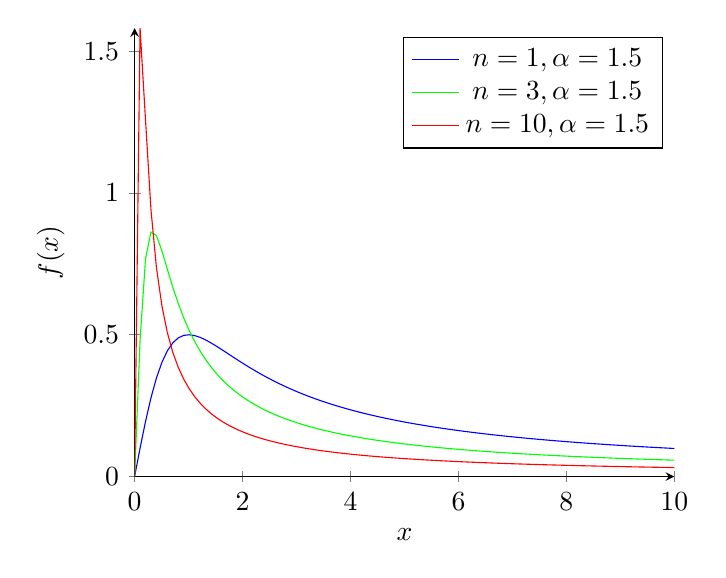
\begin{tikzpicture}
                \begin{axis}[
                        axis lines = left,
                        xlabel = $x$,
                        ylabel = {$f(x)$}
                    ]
                    \addplot [
                        domain=0:10,
                        samples=100,
                        color=blue
                    ]
                    {1^1.5 * x / (1 + 1^2 * x^2)};
                    \addlegendentry{$n=1, \alpha=1.5$}
                    \addplot [
                        domain=0:10,
                        samples=100,
                        color=green
                    ]
                    {3^1.5 * x / (1 + 3^2 * x^2)};
                    \addlegendentry{$n=3, \alpha=1.5$}
                    \addplot [
                        domain=0:10,
                        samples=100,
                        color=red
                    ]
                    {10^1.5 * x / (1 + 10^2 * x^2)};
                    \addlegendentry{$n=10, \alpha=1.5$}
                \end{axis}
            \end{tikzpicture}
        \end{minipage}
    \end{minipage}
\end{example}

\begin{definition}
    %<*равномернаясходимость>
    $f_n$ \textbf{равномерно сходится} к $f$ на $E\subset X$, если $M_n := \sup\limits_{x\in E} |f_n(x)-f(x)|\xrightarrow{n\to+\infty}0$.
    $$\forall \varepsilon \ \ \exists N \ \ \forall n > N \ \ 0\le M_n < \varepsilon \text{ т.е. } \forall x\in E \ \ |f_n(x) - f(x)| < \varepsilon$$
    Обозначается $f_n\xrightrightarrows[E]{} f$
    %</равномернаясходимость>
\end{definition}

\begin{remark}\itemfix
    \begin{itemize}
        \item $x_0\in E$
        \item $f_n \xrightrightarrows[E]{} f$
    \end{itemize}
    Тогда $f_n(x_0)\to f(x_0)$. То есть равномерная сходимость $\Rightarrow$ поточечная сходимость и предел.
\end{remark}
\begin{remark}\itemfix
    \begin{itemize}
        \item $E_0\subset E$
        \item $f_n \xrightrightarrows[E]{} f$
    \end{itemize}
    Тогда $f_n \xrightrightarrows[E_0]{} f$
\end{remark}

\begin{remark}\itemfix
    \begin{itemize}
        \item $\mathcal F = \{f : X \to \R \text{ --- огр. функции}\}$
    \end{itemize}
    Тогда $\rho(f_1, f_2) := \sup\limits_{x\in X}|f_1(x) - f_2(x)|$ --- метрика в $\mathcal F$. Называется Чебышевское расстояние.
\end{remark}
\begin{proof}
    \begin{enumerate}
        \item $\rho(f_1, f_2) \ge 0$, $\rho(f_1, f_2) = 0 \Leftrightarrow f_1\not= f_2$ --- очевидно
        \item $\rho(f_1, f_2) = \rho(f_2, f_1)$ --- очевидно
        \item $\rho(f_1, f_2) \le \rho(f_1, f_3) + \rho(f_2, f_3)$

              $\sphericalangle \varepsilon > 0 \ \ \exists x$
              \begin{align*}
                  \rho(f_1, f_2) - \varepsilon & = \sup|f_1 - f_2| - \varepsilon           \\
                                               & < |f_1(x) - f_2(x)|                       \\
                                               & \le |f_1(x) - f_3(x)| + |f_2(x) - f_3(x)| \\
                                               & \le \rho(f_1, f_3) + \rho(f_2, f_3)
              \end{align*}
    \end{enumerate}
\end{proof}

$f_n \xrightrightarrows[E]{} f \Leftrightarrow f_n \to f$ по метрике $\rho_E$.

Можем заметить, что в $\mathcal F$ при различных метриках происходит различная сходимость или расходимость, в отличие от $\R^m$.

\begin{remark}\itemfix
    \begin{itemize}
        \item $E = E_1 \cup E_2$
    \end{itemize}
    $$\begin{rcases*}
            f_n \xrightrightarrows[E_1]{} f \\
            f_n \xrightrightarrows[E_2]{} f
        \end{rcases*} \Rightarrow f_n \xrightrightarrows[E]{} f$$
\end{remark}

\end{document}

\chapter{11 октября}

\section{Гипотезы}

\begin{definition}
    \textbf{Гипотезой} \(H\) называется предположение о свойствах случайной величины.
\end{definition}

\begin{definition}
    Гипотеза называется \textbf{простой}, если она однозначно определяет распределение, т.е. \(H : \mathcal{F} = \mathcal{F}_1\), где \(\mathcal{F}_1\) --- распределение известного типа с известными параметрами.
\end{definition}

\begin{definition}
    Все остальные гипотезы называются \textbf{сложными}, т.к. они являются объединением конечного или бесконечного числа простых гипотез.
\end{definition}

\begin{definition}[основная модель гипотез]
    Гипотеза \(H_1 = \overline{H_0}\) --- конкурирующая \textit{(альтернативная)} гипотеза, состоящая в том, что основная гипотеза \(H_0\) неверна.
\end{definition}

\begin{remark}
    С помощью статистических методов нельзя \underline{доказать} гипотезу, можно только сказать, что она верна с некоторой уверенностью.
\end{remark}

Основная гипотеза \(H_0\) принимается или отклоняется с помощью \underline{статистики критерия} \(K\):
\[K(X_0 \dots X_n) \to \R = S \cup\!\footnote{Объединение на самом деле дизъюнктно.} \overline{S} \to (H_0, H_1)\]
\[\begin{cases}
        H_0, & \text{если } K \in \overline{S} \\
        H_1, & \text{если } K \in S
    \end{cases}\]

\begin{definition}
    Если точка находится на границе областей \(S\) и \(\overline{S}\), она называется \textbf{критической}.
\end{definition}

\begin{definition}
    \textbf{Ошибка I рода} состоит в том, что нулевая гипотеза отвергается, когда она верна.
\end{definition}

\begin{definition}
    \textbf{Ошибка II рода} состоит в том, что отвергается альтернативная, когда она верна.
\end{definition}

\begin{definition}
    \(\alpha\) --- вероятность ошибки II рода, \(\beta\) --- вероятность ошибки I рода/
\end{definition}

\begin{example}
    \(H_0\) --- деталь годная, \(H_1\) --- деталь бракованная.

    Ошибка I рода --- признать годную деталь бракованной.

    Ошибка II рода --- признать бракованную деталь годной.
\end{example}

\begin{remark}
    При росте выборки вероятности ошибок уменьшаются, при уменьшении вероятности одной ошибки другая вероятность увеличивается.
\end{remark}

\subsection{Способы сравнения критериев}

Пусть имеются критерии \(K_1\) и \(K_2, \alpha_1, \beta_1, \alpha_2, \beta_2\) --- вероятности ошибок при соответствующих критериях, \(h_1\) --- потери в результате ошибке I рода, \(h_2\) --- потери в результате ошибки II рода.

Тогда рассмотрим способы сравнения критериев:
\begin{enumerate}
    \item Минимакс: \(K_1\) не хуже, чем \(K_2\), если \(\max(\alpha_1 h_1, \beta_1 h_2) \leq \max(\alpha_2 h_1, \beta_2 h_2)\)
    \item Критерий называется \textbf{баесовским}, если \(U = \alpha k_1 + \beta k_2\) минимально.
    \item Пусть \(\varepsilon\) --- допустимый уровень ошибки I рода. Обозначим \(K_\varepsilon \coloneqq \{K_i \mid \alpha_i \leq \varepsilon\}\).

          \begin{definition}
              Критерий \(K \in K_\varepsilon\) называется \textbf{наиболее мощным} критерием уровня \(\varepsilon\), если \(\beta \leq \beta_i \ \ \forall i\).
          \end{definition}
\end{enumerate}

\subsection{Критерий согласия}

\begin{definition}
    Критерий \(K\) называется \textbf{критерием асимптотического уровня \(\varepsilon\)}, если вероятность ошибки первого рода \(\alpha\) стремится к \(\varepsilon\) при \(n \to \infty\).
\end{definition}

\begin{definition}
    Критерий \(K\) для проверки гипотезы \(H_0\) против альтернативы \(H_1 = \overline{H_0}\) называется \textbf{состоятельным}, если вероятность ошибки II рода \(\beta \to 0\) при \(n \to \infty\).
\end{definition}

\begin{definition}
    Критерием \textbf{согласия} уровня \(\varepsilon\) называются состоятельные критерии асимптотического уровня \(\varepsilon\).
\end{definition}

\subsection{Построение критериев согласия}

В качестве критериев согласия берётся статистика \(K(X_1 \dots X_n)\) со свойствами:
\begin{enumerate}
    \item Если \(H_0\) верна, то \(K(X_1 \dots X_n) \rightrightarrows Z\) --- известное распределение с известными параметрами.
    \item Если \(H_0\) не верна, то \(K(X_1 \dots X_n) \xrightarrow{P} \infty\)
\end{enumerate}
Для заданного уровня значимость \(\varepsilon\) находим константу \(t_k\), такую что \(P(|Z| \geq t_k) = \alpha\). В результате получаем критерий согласия уровня значимости \(\alpha = \varepsilon\):
\[\begin{cases}
        H_0, & |K| < t_k    \\
        H_1, & |K| \geq t_k
    \end{cases}\]
\begin{theorem}
    Этот критерий является критерием согласия.
\end{theorem}
\begin{proof}\itemfix
    \begin{enumerate}
        \item \(K\) --- критерий асимптотического уровня:

              Пусть \(H_0\) верна. Тогда по построению \(K \rightrightarrows Z\), т.е. \(F_K(x) \to F_Z(x)\) и
              \begin{align*}
                  \alpha & = P(|K| \geq t_k \mid H_0)                                \\
                         & = 1 - P(|K| < t_k)                                        \\
                         & = 1 - (F_K(t_k) - F_K( -t_k))                             \\
                         & \xrightarrow[n \to \infty ]{} 1 - (F_Z(t_k) - F_Z( -t_k)) \\
                         & = P(|Z| \geq t_k)                                         \\
                         & = \varepsilon
              \end{align*}
        \item \(K\) --- состоятельный критерий:

              Пусть \(H_1\) верна. Тогда \(K(X_1 \dots X_n) \xrightarrow[]{P} \infty\), т.е.
              \[\forall C \ \ P(|K| \geq C \mid H_1) \xrightarrow[n \to \infty ]{P} 1 \Rightarrow \beta = P(|K| < t_k \mid H_1) \xrightarrow[n \to \infty ]{P} 0\]
    \end{enumerate}
\end{proof}

\begin{exercise*}
    Гипотеза о среднем нормальной совокупности с известной дисперсией.

    Пусть имеется выборка \((X_1 \dots X_n) \in X \in N(a, \sigma^2)\), причём второй параметр известен.\footnote{Например, мы измеряем что-то инструментом заданной точности.}

    \(H_0: a = a_0, H_1 : a \neq a_0\).

    В качестве статистики критерия возьмём \(\sqrt{n} \cdot \frac{ \overline{X} - a_0}{\sigma}\). Проверим, что оно имеет требуемые свойства:
    \begin{enumerate}
        \item Если \(H_0\) верна, т.е. \(a = a_0\), то \(\sqrt{n} \frac{ \overline{X} - a_0}{\sigma} = \sqrt{n} \frac{ \overline{X} - a}{\sigma} \in N(0, 1)\)
        \item Если \(H_0\) неверно, т.е. \(a \neq a_0\), то \(|K| \to \infty \):

              \[|K| = \left|\sqrt{n} \frac{ \overline{X} - a_0}{\sigma}\right|= \underbrace{\sqrt{n}}_{ \to \infty } \left|\underbrace{\frac{ \overline{X} - a}{\sigma}}_{\in N(0, 1)} + \underbrace{\frac{a - a_0}{\sigma}}_{\neq 0}\right| \xrightarrow[n \to \infty ]{P} \infty\]
    \end{enumerate}

    Таким образом, этот критерий --- критерий согласия. Для уровня значимости \(\alpha = \varepsilon\) выберем \(C\), такую что \(\varepsilon = P(|K| \geq C) \Rightarrow P(|K| < C) = 1 - \varepsilon \Rightarrow 2 \Phi(C) = 1 - \varepsilon \Rightarrow 2 \Phi(C) = \frac{1 - \varepsilon}{2}\)

    Итого:
    \[\begin{cases}
            H_0, & |K| = \left|\sqrt{n} \frac{ \overline{X} - a_0}{\sigma}\right| < C    \\
            H_1, & |K| = \left|\sqrt{n} \frac{ \overline{X} - a_0}{\sigma}\right| \geq C
        \end{cases}\]
    Заметим, что если мы решим это неравенство, то получим доверительный интервал для параметра \(a\) нормального распределения при известном \(\sigma\).
\end{exercise*}

\begin{remark}
    Аналогично можно проверять для неизвестного \(\sigma\), тогда в критерии \(\sigma\) заменится на \(S\).
\end{remark}

\subsection{Доверительные интервалы как критерии гипотез о параметрах распределения}

Пусть имеется выборка \((X_1 \dots X_n)\) случайной величины \(X \in \mathcal{F}_\theta\), где \(\mathcal{F}_\theta\) --- распределение известного типа с неизвестным параметром \(\theta\). Проверяется гипотеза: \(H_0 : \theta = \theta_0\) против \(H_1 : \theta \neq \theta_0\). Пусть для \(\theta\) построен доверительный интервал \((\theta^- , \theta^+)\) надежности \(\gamma\). Тогда следующий критерий является критерием согласия уровня \(\alpha = 1 - \gamma\):
\[\begin{cases}
        H_0, & \theta_0 \in (\theta^- , \theta^+)    \\
        H_1, & \theta_0 \notin (\theta^- , \theta^+)
    \end{cases}\]
\begin{proof}
    \[\alpha = P(\theta_0 \notin (\theta^- , \theta^+) \mid X \in \mathcal{F}_\theta) = 1 - P(\theta_0 \in (\theta^- , \theta^+) \mid X \in \mathcal{F}_\theta) = 1 - \gamma = \alpha\]

    Доказывать состоятельность критерия нужно в каждом случае отдельно.
\end{proof}

\begin{example}
    По выборке объема \(n = 36\) из нормальной совокупности с известным \(\sigma = 1.44\) найдено выборочное среднее \(\overline{X} = 21.36\). Проверить гипотезу \(H_0 : a = 21\) против \(H_1 : a \neq 21\) при уровне значимости \(\alpha = 0.05\).
    \[K = \sqrt{n} \frac{ \overline{X} - a_0}{\sigma} = \sqrt{36} \frac{21.6 - 21}{1.44} = 2.5\]
    \[\Phi(t_k) = \frac{1 - \alpha}{2} = 0.475\]
    \[t_k = 1.96\]
    Т.к. \(|K| = 2.5 > 1.96\), гипотеза отклоняется.
\end{example}

В математических пакетах могут не сравнивать с критической точкой, а считать статистику и искать вероятность.

\begin{remark}
    Следующий материал был рассказан на практике 13 октября.
\end{remark}

\subsection{Распределение Коши}

Пусть дан источник некоторого излучения в точке \((0, 1)\), который равномерно посылает лучи во все стороны.

Случайная величина \(\xi\) --- точка пересечения луча с осью \(OX\).

Найти \(F_\xi(x), f_\xi(x), \E \xi\).

\begin{figure}[h]
    \centering
    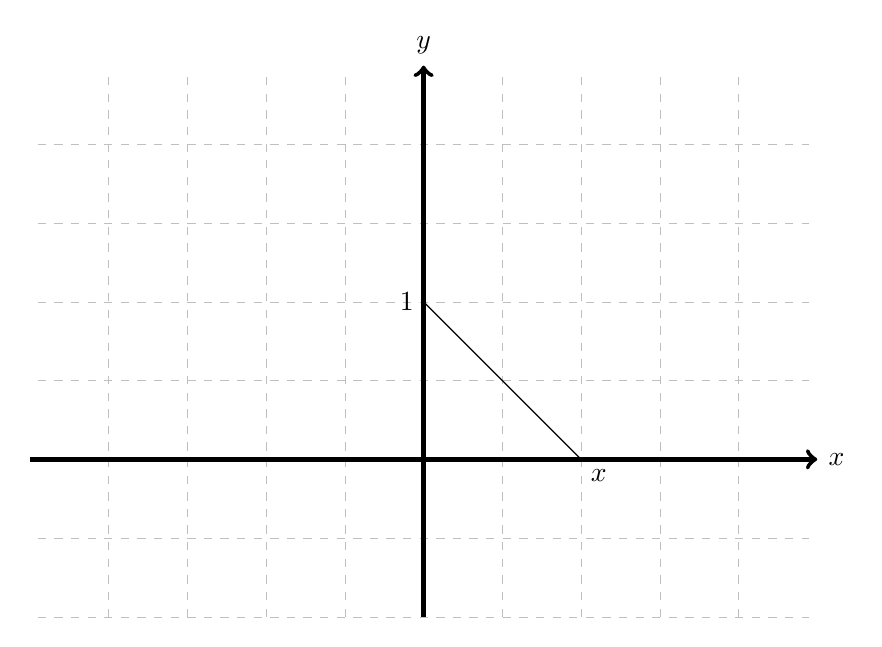
\begin{tikzpicture}
        \draw[help lines, color=gray!50, dashed] (-4.9,-2) grid (4.9,4.9);
        \draw[->,ultra thick] (-5,0)--(5,0) node[right]{$x$};
        \draw[->,ultra thick] (0,-2)--(0,5) node[above]{$y$};
        \draw (0, 2) node[left] {1} -- (2, 0);
        \node[below right] at (2, 0) {\(x\)};
        % \draw (0, 2) arc (180:360:0.1);
    \end{tikzpicture}
    \caption{Источник}
\end{figure}

\[F_\xi(x) = P(\xi < x) = P(\xi < 0) + P(0 < \xi < x) = 0.5 + \frac{1}{\pi} \arctg x\]
\[f_\xi(x) = F_\xi'(x) = \frac{1}{\pi} \frac{1}{x^2 + 1}\]
\[\E \xi = \int_{ - \infty }^{ + \infty } x f_\xi(x) = \int_{ - \infty }^{ + \infty } x \frac{1}{\pi} \frac{1}{x^2 + 1} dx = \frac{1}{2 \pi} \ln(1 + x^2) \Big|_{ - \infty }^{ + \infty}, \nexists\]

Пусть теперь источник сдвинут на \(\theta\) по оси \(x\). Тогда \(f_\xi(x) = \frac{1}{\pi (1 + (x - \theta)^2)}\). Попробуем оценить \(\theta\). \(\overline{X}\) не работает, т.к. оно убежит на бесконечность: \(\E \frac{S_n}{n} = \E X\). Оценим с помощью медианы. По симметрии \(\theta = \mathrm{Me} \xi\).

\[\mathrm{Me}^* = \begin{cases}
        X_{(k + 1)},                     & n = 2k + 1 \\
        \frac{X_{(k)} + X_{(k + 1)}}{2}, & n = 2k
    \end{cases}\]

\begin{theorem}
    Если \(f(\mathrm{Me}) \neq 0\), то \(\mathrm{Me}^* \xrightarrow{P} \mathrm{Me}\), причём сходится со скоростью \(\frac{1}{\sqrt{n}}\).
\end{theorem}

В целом при большом числе выбросов медиана помогает. Например, оценивать зарплату нужно по медиане, а не по среднему.

У медианы также есть свои недостатки: она сходится медленнее, чем выборочное среднее --- эффективность обычно ниже на 20-30\%, но бывают и случаи хуже.

Есть и другие оценки, например \textbf{усечённое среднее}. Выкидываются наименьшие и наибольшие \(k\) точек и считается выборочное среднее:
\[\frac{\sum\limits_{i= k + 1}^{n - k} X_{(i)}}{n - 2k}\]
Несложно заметить, что это нечто промежуточное между выборочным средним и медианой --- если \(k = 0\), то получаем выборочное среднее, если \(k = \frac{n - 1}{2}\), то получаем медиану.

Другой пример: составим по исходной выборке выборку объема \(\frac{n(n - 1)}{2}\), состоящую из \(\frac{X_i + X_j}{2}, 1 \leq i,j \leq n\). \textbf{Среднее Уолша} --- медиана этой выборки. У этой оценки эффективность падает на \(\approx 12\%\) относительно выборочного среднего.

\begin{exercise}
    Дано \(n\) призывников с вероятностью болезни \(p = 0.01\). Разбиваем призывников на группы по \(k\) человек в группе. Считаем, что \(n \divided k\), т.е. групп \(\frac{n}{k}\). В каждой группе:
    \begin{itemize}
        \item Если суммарный результат отрицательный, то \(1\) анализ.
        \item Иначе \(k + 1\) анализ.
    \end{itemize}

    Найти оптимиальное значение \(k\) и среднее значение числа анализов.
\end{exercise}
\begin{solution}
    \(\xi_i\) --- число анализов в \(i\)-той группе.

    \[P(\xi_i = 1) = (1 - p)^k \quad P(\xi_i = k + 1) = 1 - (1 - p)^k\]
    \[\E \xi_i = (1 - p)^k + (k + 1)(1 - (1 - p)^k) = k + 1 - k(1 - p)^k\]
    \[\xi = \frac{n}{k} \cdot \xi_i\]
    \[\E \xi = n\left(1 + \frac{1}{k} - (1 - p)^k\right) = f(k)\]
    Т.к. \(p\) мало, пусть оно \(p \to 0\). \((1 - p)^k \sim 1 - pk\).
    \[f(k) \sim n \left(\frac{1}{k} + pk\right)\]
    \[f'(k) = n \left( - \frac{1}{k^2} + p \right) = 0\]
    \[k = \frac{1}{\sqrt{p}} = 10\]
    \[\E \xi \approx n \left(\frac{1}{10} + 0.01 \cdot 10\right) = 0.2 n\]
\end{solution}

\documentclass[12pt, a4paper]{article}

%<*preamble>
% Math symbols
\usepackage{amsmath, amsthm, amsfonts, amssymb}
\usepackage{accents}
\usepackage{esvect}
\usepackage{mathrsfs}
\usepackage{mathtools}
\mathtoolsset{showonlyrefs}
\usepackage{cmll}
\usepackage{stmaryrd}
\usepackage{physics}
\usepackage[normalem]{ulem}
\usepackage{ebproof}
\usepackage{extarrows}

% Page layout
\usepackage{geometry, a4wide, parskip, fancyhdr}

% Font, encoding, russian support
\usepackage[russian]{babel}
\usepackage[sb]{libertine}
\usepackage{xltxtra}

% Listings
\usepackage{listings}
\lstset{basicstyle=\ttfamily,breaklines=true}
\setmonofont{Inconsolata}

% Miscellaneous
\usepackage{array}
\usepackage{calc}
\usepackage{caption}
\usepackage{subcaption}
\captionsetup{justification=centering,margin=2cm}
\usepackage{catchfilebetweentags}
\usepackage{enumitem}
\usepackage{etoolbox}
\usepackage{float}
\usepackage{lastpage}
\usepackage{minted}
\usepackage{svg}
\usepackage{wrapfig}
\usepackage{xcolor}
\usepackage[makeroom]{cancel}

\newcolumntype{L}{>{$}l<{$}}
    \newcolumntype{C}{>{$}c<{$}}
\newcolumntype{R}{>{$}r<{$}}

% Footnotes
\usepackage[hang]{footmisc}
\setlength{\footnotemargin}{2mm}
\makeatletter
\def\blfootnote{\gdef\@thefnmark{}\@footnotetext}
\makeatother

% References
\usepackage{hyperref}
\hypersetup{
    colorlinks,
    linkcolor={blue!80!black},
    citecolor={blue!80!black},
    urlcolor={blue!80!black},
}

% tikz
\usepackage{tikz}
\usepackage{tikz-cd}
\usetikzlibrary{arrows.meta}
\usetikzlibrary{decorations.pathmorphing}
\usetikzlibrary{calc}
\usetikzlibrary{patterns}
\usepackage{pgfplots}
\pgfplotsset{width=10cm,compat=1.9}
\newcommand\irregularcircle[2]{% radius, irregularity
    \pgfextra {\pgfmathsetmacro\len{(#1)+rand*(#2)}}
    +(0:\len pt)
    \foreach \a in {10,20,...,350}{
            \pgfextra {\pgfmathsetmacro\len{(#1)+rand*(#2)}}
            -- +(\a:\len pt)
        } -- cycle
}

\providetoggle{useproofs}
\settoggle{useproofs}{false}

\pagestyle{fancy}
\lfoot{M3137y2019}
\cfoot{}
\rhead{стр. \thepage\ из \pageref*{LastPage}}

\newcommand{\R}{\mathbb{R}}
\newcommand{\Q}{\mathbb{Q}}
\newcommand{\Z}{\mathbb{Z}}
\newcommand{\B}{\mathbb{B}}
\newcommand{\N}{\mathbb{N}}
\renewcommand{\Re}{\mathfrak{R}}
\renewcommand{\Im}{\mathfrak{I}}

\newcommand{\const}{\text{const}}
\newcommand{\cond}{\text{cond}}

\newcommand{\teormin}{\textcolor{red}{!}\ }

\DeclareMathOperator*{\xor}{\oplus}
\DeclareMathOperator*{\equ}{\sim}
\DeclareMathOperator{\sign}{\text{sign}}
\DeclareMathOperator{\Sym}{\text{Sym}}
\DeclareMathOperator{\Asym}{\text{Asym}}

\DeclarePairedDelimiter{\ceil}{\lceil}{\rceil}

% godel
\newbox\gnBoxA
\newdimen\gnCornerHgt
\setbox\gnBoxA=\hbox{$\ulcorner$}
\global\gnCornerHgt=\ht\gnBoxA
\newdimen\gnArgHgt
\def\godel #1{%
    \setbox\gnBoxA=\hbox{$#1$}%
    \gnArgHgt=\ht\gnBoxA%
    \ifnum     \gnArgHgt<\gnCornerHgt \gnArgHgt=0pt%
    \else \advance \gnArgHgt by -\gnCornerHgt%
    \fi \raise\gnArgHgt\hbox{$\ulcorner$} \box\gnBoxA %
    \raise\gnArgHgt\hbox{$\urcorner$}}

% \theoremstyle{plain}

\theoremstyle{definition}
\newtheorem{theorem}{Теорема}
\newtheorem*{definition}{Определение}
\newtheorem{axiom}{Аксиома}
\newtheorem*{axiom*}{Аксиома}
\newtheorem{lemma}{Лемма}

\theoremstyle{remark}
\newtheorem*{remark}{Примечание}
\newtheorem*{exercise}{Упражнение}
\newtheorem{corollary}{Следствие}[theorem]
\newtheorem*{statement}{Утверждение}
\newtheorem*{corollary*}{Следствие}
\newtheorem*{example}{Пример}
\newtheorem{observation}{Наблюдение}
\newtheorem*{prop}{Свойства}
\newtheorem*{obozn}{Обозначение}

% subtheorem
\makeatletter
\newenvironment{subtheorem}[1]{%
    \def\subtheoremcounter{#1}%
    \refstepcounter{#1}%
    \protected@edef\theparentnumber{\csname the#1\endcsname}%
    \setcounter{parentnumber}{\value{#1}}%
    \setcounter{#1}{0}%
    \expandafter\def\csname the#1\endcsname{\theparentnumber.\Alph{#1}}%
    \ignorespaces
}{%
    \setcounter{\subtheoremcounter}{\value{parentnumber}}%
    \ignorespacesafterend
}
\makeatother
\newcounter{parentnumber}

\newtheorem{manualtheoreminner}{Теорема}
\newenvironment{manualtheorem}[1]{%
    \renewcommand\themanualtheoreminner{#1}%
    \manualtheoreminner
}{\endmanualtheoreminner}

\newcommand{\dbltilde}[1]{\accentset{\approx}{#1}}
\newcommand{\intt}{\int\!}

% magical thing that fixes paragraphs
\makeatletter
\patchcmd{\CatchFBT@Fin@l}{\endlinechar\m@ne}{}
{}{\typeout{Unsuccessful patch!}}
\makeatother

\newcommand{\get}[2]{
    \ExecuteMetaData[#1]{#2}
}

\newcommand{\getproof}[2]{
    \iftoggle{useproofs}{\ExecuteMetaData[#1]{#2proof}}{}
}

\newcommand{\getwithproof}[2]{
    \get{#1}{#2}
    \getproof{#1}{#2}
}

\newcommand{\import}[3]{
    \subsection{#1}
    \getwithproof{#2}{#3}
}

\newcommand{\given}[1]{
    Дано выше. (\ref{#1}, стр. \pageref{#1})
}

\renewcommand{\ker}{\text{Ker }}
\newcommand{\im}{\text{Im }}
\renewcommand{\grad}{\text{grad}}
\newcommand{\rg}{\text{rg}}
\newcommand{\defeq}{\stackrel{\text{def}}{=}}
\newcommand{\defeqfor}[1]{\stackrel{\text{def } #1}{=}}
\newcommand{\itemfix}{\leavevmode\makeatletter\makeatother}
\newcommand{\?}{\textcolor{red}{???}}
\renewcommand{\emptyset}{\varnothing}
\newcommand{\longarrow}[1]{\xRightarrow[#1]{\qquad}}
\DeclareMathOperator*{\esup}{\text{ess sup}}
\newcommand\smallO{
    \mathchoice
    {{\scriptstyle\mathcal{O}}}% \displaystyle
    {{\scriptstyle\mathcal{O}}}% \textstyle
    {{\scriptscriptstyle\mathcal{O}}}% \scriptstyle
    {\scalebox{.6}{$\scriptscriptstyle\mathcal{O}$}}%\scriptscriptstyle
}
\renewcommand{\div}{\text{div}\ }
\newcommand{\rot}{\text{rot}\ }
\newcommand{\cov}{\text{cov}}

\makeatletter
\newcommand{\oplabel}[1]{\refstepcounter{equation}(\theequation\ltx@label{#1})}
\makeatother

\newcommand{\symref}[2]{\stackrel{\oplabel{#1}}{#2}}
\newcommand{\symrefeq}[1]{\symref{#1}{=}}

% xrightrightarrows
\makeatletter
\newcommand*{\relrelbarsep}{.386ex}
\newcommand*{\relrelbar}{%
    \mathrel{%
        \mathpalette\@relrelbar\relrelbarsep
    }%
}
\newcommand*{\@relrelbar}[2]{%
    \raise#2\hbox to 0pt{$\m@th#1\relbar$\hss}%
    \lower#2\hbox{$\m@th#1\relbar$}%
}
\providecommand*{\rightrightarrowsfill@}{%
    \arrowfill@\relrelbar\relrelbar\rightrightarrows
}
\providecommand*{\leftleftarrowsfill@}{%
    \arrowfill@\leftleftarrows\relrelbar\relrelbar
}
\providecommand*{\xrightrightarrows}[2][]{%
    \ext@arrow 0359\rightrightarrowsfill@{#1}{#2}%
}
\providecommand*{\xleftleftarrows}[2][]{%
    \ext@arrow 3095\leftleftarrowsfill@{#1}{#2}%
}

\allowdisplaybreaks

\newcommand{\unfinished}{\textcolor{red}{Не дописано}}

% Reproducible pdf builds 
\special{pdf:trailerid [
<00112233445566778899aabbccddeeff>
<00112233445566778899aabbccddeeff>
]}
%</preamble>


\lhead{Матстат \textit{(практика)}}
\cfoot{}
\rfoot{22.10.2021}

\begin{document}

Все вычисления доступны по \href{https://docs.google.com/spreadsheets/d/1lU-0FnVcjXLhWT8c0K_v2xk-lVkF9Ary3zV-o6R1Was/edit?usp=sharing}{ссылке}, листы ``7.1'' и ``7.2''.

\begin{exercise}
    Проверить, что распределение второй величины нормально с уверенностью \(\alpha = 0.05\).
\end{exercise}

Мы объединяем интервалы таким образом, чтобы в каждом интервале было хотя бы \(5\) точек.

\[P(a_i < \xi < a_{i+1}) = F(a_{i+1}) - F(a_i) = \Phi\left(\frac{a_{i+1} - a}{\sigma}\right) - \Phi\left(\frac{a_i - a}{\sigma}\right) = \Phi\left(\frac{a_{i+1} - \overline{X}}{S}\right) - \Phi(\frac{a_i - \overline{X}}{S})\]
Число степеней свободы \(s = k\) \textit{(число интервалов)} \(- m\) \textit{(число параметров распределения)} \(- 1 = 1\)
Т.к. \(\chi\) практическое \( = 0.49 < \chi\) теоретическое \( = \text{ХИ2.ОБР.2Х}(\alpha, s) = 3.84\), гипотеза принимается.

\begin{exercise}
    Проверить, что распределение первой величины экспоненциально с уверенностью \(\alpha = 0.05\).
\end{exercise}

Все так же, но \(F(a_i) = \exp( - \alpha a_i)\) и \(\alpha^* = \frac{1}{\overline{X}}\). \(\chi_{\text{практ.}} = 23.45 > \chi_{\text{теор.}} = 7.81\), гипотеза отклоняется.

\begin{exercise}
    Среди населения \(1\%\) воров. В комнате из \(10\) человек пропал кошелек. Какова вероятность того, что случайно выбранный из комнаты человек --- вор?
\end{exercise}

\end{document}

\documentclass[12pt, a4paper]{article}

%<*preamble>
% Math symbols
\usepackage{amsmath, amsthm, amsfonts, amssymb}
\usepackage{accents}
\usepackage{esvect}
\usepackage{mathrsfs}
\usepackage{mathtools}
\mathtoolsset{showonlyrefs}
\usepackage{cmll}
\usepackage{stmaryrd}
\usepackage{physics}
\usepackage[normalem]{ulem}
\usepackage{ebproof}
\usepackage{extarrows}

% Page layout
\usepackage{geometry, a4wide, parskip, fancyhdr}

% Font, encoding, russian support
\usepackage[russian]{babel}
\usepackage[sb]{libertine}
\usepackage{xltxtra}

% Listings
\usepackage{listings}
\lstset{basicstyle=\ttfamily,breaklines=true}
\setmonofont{Inconsolata}

% Miscellaneous
\usepackage{array}
\usepackage{calc}
\usepackage{caption}
\usepackage{subcaption}
\captionsetup{justification=centering,margin=2cm}
\usepackage{catchfilebetweentags}
\usepackage{enumitem}
\usepackage{etoolbox}
\usepackage{float}
\usepackage{lastpage}
\usepackage{minted}
\usepackage{svg}
\usepackage{wrapfig}
\usepackage{xcolor}
\usepackage[makeroom]{cancel}

\newcolumntype{L}{>{$}l<{$}}
    \newcolumntype{C}{>{$}c<{$}}
\newcolumntype{R}{>{$}r<{$}}

% Footnotes
\usepackage[hang]{footmisc}
\setlength{\footnotemargin}{2mm}
\makeatletter
\def\blfootnote{\gdef\@thefnmark{}\@footnotetext}
\makeatother

% References
\usepackage{hyperref}
\hypersetup{
    colorlinks,
    linkcolor={blue!80!black},
    citecolor={blue!80!black},
    urlcolor={blue!80!black},
}

% tikz
\usepackage{tikz}
\usepackage{tikz-cd}
\usetikzlibrary{arrows.meta}
\usetikzlibrary{decorations.pathmorphing}
\usetikzlibrary{calc}
\usetikzlibrary{patterns}
\usepackage{pgfplots}
\pgfplotsset{width=10cm,compat=1.9}
\newcommand\irregularcircle[2]{% radius, irregularity
    \pgfextra {\pgfmathsetmacro\len{(#1)+rand*(#2)}}
    +(0:\len pt)
    \foreach \a in {10,20,...,350}{
            \pgfextra {\pgfmathsetmacro\len{(#1)+rand*(#2)}}
            -- +(\a:\len pt)
        } -- cycle
}

\providetoggle{useproofs}
\settoggle{useproofs}{false}

\pagestyle{fancy}
\lfoot{M3137y2019}
\cfoot{}
\rhead{стр. \thepage\ из \pageref*{LastPage}}

\newcommand{\R}{\mathbb{R}}
\newcommand{\Q}{\mathbb{Q}}
\newcommand{\Z}{\mathbb{Z}}
\newcommand{\B}{\mathbb{B}}
\newcommand{\N}{\mathbb{N}}
\renewcommand{\Re}{\mathfrak{R}}
\renewcommand{\Im}{\mathfrak{I}}

\newcommand{\const}{\text{const}}
\newcommand{\cond}{\text{cond}}

\newcommand{\teormin}{\textcolor{red}{!}\ }

\DeclareMathOperator*{\xor}{\oplus}
\DeclareMathOperator*{\equ}{\sim}
\DeclareMathOperator{\sign}{\text{sign}}
\DeclareMathOperator{\Sym}{\text{Sym}}
\DeclareMathOperator{\Asym}{\text{Asym}}

\DeclarePairedDelimiter{\ceil}{\lceil}{\rceil}

% godel
\newbox\gnBoxA
\newdimen\gnCornerHgt
\setbox\gnBoxA=\hbox{$\ulcorner$}
\global\gnCornerHgt=\ht\gnBoxA
\newdimen\gnArgHgt
\def\godel #1{%
    \setbox\gnBoxA=\hbox{$#1$}%
    \gnArgHgt=\ht\gnBoxA%
    \ifnum     \gnArgHgt<\gnCornerHgt \gnArgHgt=0pt%
    \else \advance \gnArgHgt by -\gnCornerHgt%
    \fi \raise\gnArgHgt\hbox{$\ulcorner$} \box\gnBoxA %
    \raise\gnArgHgt\hbox{$\urcorner$}}

% \theoremstyle{plain}

\theoremstyle{definition}
\newtheorem{theorem}{Теорема}
\newtheorem*{definition}{Определение}
\newtheorem{axiom}{Аксиома}
\newtheorem*{axiom*}{Аксиома}
\newtheorem{lemma}{Лемма}

\theoremstyle{remark}
\newtheorem*{remark}{Примечание}
\newtheorem*{exercise}{Упражнение}
\newtheorem{corollary}{Следствие}[theorem]
\newtheorem*{statement}{Утверждение}
\newtheorem*{corollary*}{Следствие}
\newtheorem*{example}{Пример}
\newtheorem{observation}{Наблюдение}
\newtheorem*{prop}{Свойства}
\newtheorem*{obozn}{Обозначение}

% subtheorem
\makeatletter
\newenvironment{subtheorem}[1]{%
    \def\subtheoremcounter{#1}%
    \refstepcounter{#1}%
    \protected@edef\theparentnumber{\csname the#1\endcsname}%
    \setcounter{parentnumber}{\value{#1}}%
    \setcounter{#1}{0}%
    \expandafter\def\csname the#1\endcsname{\theparentnumber.\Alph{#1}}%
    \ignorespaces
}{%
    \setcounter{\subtheoremcounter}{\value{parentnumber}}%
    \ignorespacesafterend
}
\makeatother
\newcounter{parentnumber}

\newtheorem{manualtheoreminner}{Теорема}
\newenvironment{manualtheorem}[1]{%
    \renewcommand\themanualtheoreminner{#1}%
    \manualtheoreminner
}{\endmanualtheoreminner}

\newcommand{\dbltilde}[1]{\accentset{\approx}{#1}}
\newcommand{\intt}{\int\!}

% magical thing that fixes paragraphs
\makeatletter
\patchcmd{\CatchFBT@Fin@l}{\endlinechar\m@ne}{}
{}{\typeout{Unsuccessful patch!}}
\makeatother

\newcommand{\get}[2]{
    \ExecuteMetaData[#1]{#2}
}

\newcommand{\getproof}[2]{
    \iftoggle{useproofs}{\ExecuteMetaData[#1]{#2proof}}{}
}

\newcommand{\getwithproof}[2]{
    \get{#1}{#2}
    \getproof{#1}{#2}
}

\newcommand{\import}[3]{
    \subsection{#1}
    \getwithproof{#2}{#3}
}

\newcommand{\given}[1]{
    Дано выше. (\ref{#1}, стр. \pageref{#1})
}

\renewcommand{\ker}{\text{Ker }}
\newcommand{\im}{\text{Im }}
\renewcommand{\grad}{\text{grad}}
\newcommand{\rg}{\text{rg}}
\newcommand{\defeq}{\stackrel{\text{def}}{=}}
\newcommand{\defeqfor}[1]{\stackrel{\text{def } #1}{=}}
\newcommand{\itemfix}{\leavevmode\makeatletter\makeatother}
\newcommand{\?}{\textcolor{red}{???}}
\renewcommand{\emptyset}{\varnothing}
\newcommand{\longarrow}[1]{\xRightarrow[#1]{\qquad}}
\DeclareMathOperator*{\esup}{\text{ess sup}}
\newcommand\smallO{
    \mathchoice
    {{\scriptstyle\mathcal{O}}}% \displaystyle
    {{\scriptstyle\mathcal{O}}}% \textstyle
    {{\scriptscriptstyle\mathcal{O}}}% \scriptstyle
    {\scalebox{.6}{$\scriptscriptstyle\mathcal{O}$}}%\scriptscriptstyle
}
\renewcommand{\div}{\text{div}\ }
\newcommand{\rot}{\text{rot}\ }
\newcommand{\cov}{\text{cov}}

\makeatletter
\newcommand{\oplabel}[1]{\refstepcounter{equation}(\theequation\ltx@label{#1})}
\makeatother

\newcommand{\symref}[2]{\stackrel{\oplabel{#1}}{#2}}
\newcommand{\symrefeq}[1]{\symref{#1}{=}}

% xrightrightarrows
\makeatletter
\newcommand*{\relrelbarsep}{.386ex}
\newcommand*{\relrelbar}{%
    \mathrel{%
        \mathpalette\@relrelbar\relrelbarsep
    }%
}
\newcommand*{\@relrelbar}[2]{%
    \raise#2\hbox to 0pt{$\m@th#1\relbar$\hss}%
    \lower#2\hbox{$\m@th#1\relbar$}%
}
\providecommand*{\rightrightarrowsfill@}{%
    \arrowfill@\relrelbar\relrelbar\rightrightarrows
}
\providecommand*{\leftleftarrowsfill@}{%
    \arrowfill@\leftleftarrows\relrelbar\relrelbar
}
\providecommand*{\xrightrightarrows}[2][]{%
    \ext@arrow 0359\rightrightarrowsfill@{#1}{#2}%
}
\providecommand*{\xleftleftarrows}[2][]{%
    \ext@arrow 3095\leftleftarrowsfill@{#1}{#2}%
}

\allowdisplaybreaks

\newcommand{\unfinished}{\textcolor{red}{Не дописано}}

% Reproducible pdf builds 
\special{pdf:trailerid [
<00112233445566778899aabbccddeeff>
<00112233445566778899aabbccddeeff>
]}
%</preamble>


\lhead{Математический анализ}
\cfoot{}
\rfoot{2.11.2020}

\begin{document}

\subsection*{Потенциальные векторные поля}

\begin{definition}
    Интеграл векторного поля $V$ \textbf{не зависит от пути} в области $O$:

    $\forall A, B\in O \ \ \forall \gamma_1, \gamma_2$ --- кусочно-гладкие из $A$ в $B$:
    $$\int_{\gamma_1} \sum v_i dx_i = \int_{\gamma_2} \sum v_i dx_i$$
\end{definition}

\begin{theorem}[характеризация потенциальных векторных полей в терминах интегралов]
    %<*характеризацияпотенциальныхвекторныхполейвтерминахинтегралов>
    $V$ --- векторное поле в области $O$. Тогда эквивалентны следующие:
    \begin{enumerate}
        \item $V$ --- потенциально
        \item $\int_\gamma \sum v_i dx_i$ не зависит от пути в $O$
        \item $\forall \gamma$ --- кусочно-гладкий, замкнутый в $O$ $\int_\gamma \sum v_i dx_i = 0$
    \end{enumerate}
    %</характеризацияпотенциальныхвекторныхполейвтерминахинтегралов>
\end{theorem}
%<*характеризацияпотенциальныхвекторныхполейвтерминахинтеграловproof>
\begin{proof}\itemfix
    \begin{itemize}
        \item [1$\Rightarrow$2] Обобщенная формула Ньютона-Лейбница
        \item [2$\Rightarrow$3] $\gamma$ --- петля: $[a, b]\to O$. $\gamma(a) = \gamma(b) = A$

              Рассмотрим постоянный путь $\tilde \gamma : [a, b]\to 0, t\mapsto A$. По свойству 2: $\int_\gamma = \int_{\tilde \gamma} \langle V, \gamma' \rangle dt = 0$
        \item [3$\Rightarrow$2] $\gamma_1, \gamma_2$ --- пути с общим началом и концом. Тогда $\gamma := \gamma_2^- \gamma_1$ --- петля. $\gamma$ --- кусочно гладкий $\Rightarrow \int_\gamma = 0$

              \begin{figure}[h]
                  \centering
                  \includesvg[scale=1]{images/характеризацияпотенциальныхполей32.svg}
              \end{figure}
        \item [2$\Rightarrow$1] Фиксируем $A\in O$.

              $\forall x\in O$ выберем кусочно-гладкий путь $\gamma_x$ из $A$ в $x$. Проверим, что $f(x) := \int_{\gamma_x} \sum v_i dx_i$ --- потенциал.

              Достаточно проверить, что $\cfrac{\partial f}{\partial x_1} = V_1$ в $O$.

              Фиксируем $x\in O$. $\gamma_0(t) = x + th e_1, t\in[0, 1]$, $\gamma_0'(t) = (h, 0 \ldots 0) = he_1$

              \begin{figure}[h]
                  \centering
                  \includesvg[scale=0.7]{images/pot_vfield_char.svg}
              \end{figure}

              \begin{align*}
                  f(x + he_1) - f(x) & = \int_{\gamma_{x+he_1}} - \int_{\gamma_x}  \\
                                     & = \int_{\gamma_0\gamma_x} - \int_{\gamma_x} \\
                                     & = \int_{\gamma_0}                           \\
                                     & = \int_0^1 V_1(\gamma_0(t)) hdt             \\
                                     & = h V_1(x_1 + ch_1, x_2 \ldots x_n)
              \end{align*}

              Таким образом:
              $$\frac{f(x + he_1) - f(x)}{h} \xrightarrow{h\to0} V_1(x_1 + ch_1, x_2 \ldots x_n) \xrightarrow{h\to0} V_1(x)$$
    \end{itemize}
\end{proof}
%</характеризацияпотенциальныхвекторныхполейвтерминахинтеграловproof>

\subsection*{Локально-потенциальные векторные поля}

\begin{lemma}
    %<*необходимоеусловиепотенциальности>
    $V$ --- гладкое, потенциальное в $O$

    Тогда
    \begin{equation}
        \forall x\in O \ \ \forall k,j \ \ \frac{\partial V_k}{\partial x_j}(x) = \frac{\partial V_j}{\partial x_k}(x) \label{производные поля}
    \end{equation}
    %</необходимоеусловиепотенциальности>
\end{lemma}
%<*необходимоеусловиепотенциальностиproof>
\begin{proof}
    Непрерывные производные не изменяются при порядке дифференцирования:
    $$\frac{\partial V_k}{\partial x_j}(x) = \frac{\partial^2 f}{\partial x_k \partial x_j}(x) = \frac{\partial^2 f}{\partial x_j \partial x_k}(x) = \frac{\partial V_j}{\partial x_k}(x)$$
\end{proof}
%</необходимоеусловиепотенциальностиproof>

\begin{exercise}
    Даны 4 векторных поля в $\R^2$: $(x, y), (x, -y), (y, x), (-y, x)$. Вычеркните лишнее.

    Ответ: \( (- y, x)\), т.к. \(\frac{\partial V_1}{\partial y} = - 1 \neq \frac{\partial V_2}{\partial x} = 1\)
\end{exercise}

\begin{theorem}[лемма Пуанкаре]\itemfix
    %<*леммапуанкаре>
    \begin{itemize}
        \item $O\subset \R^m$ --- \textbf{выпуклая} область
        \item $V : O\to\R^m$ --- векторное поле
        \item $V$ удовлетворяет \ref{производные поля}, в т.ч. $V$ --- гладкое.
    \end{itemize}
    Тогда $V$ --- потенциальное.
    %</леммапуанкаре>
\end{theorem}
%<*леммапуанкареproof>
\begin{proof}
    Фиксируем $A\in O$
    $$\forall x\in O \ \ \gamma_x(t) := A + t(x-A), t\in[0, 1]$$
    $$\gamma'_x(t) = x - A$$
    $$f(x) := \int_{\gamma_x} \sum v_i dx_i = \int_0^1 \sum_{k=1}^m V_k(A+t(x-A))(x_k - A_k)dt$$
    Проверим, что $f$ --- потенциал.
    \begin{align}
        \frac{\partial f}{\partial x_j} (x) & = \text{правило Лейбница}                                                                      \nonumber                         \\
                                            & = \int_0^1 V_j(A + t(x-A)) + \sum_{k=1}^m \frac{\partial V_k}{\partial x_j}(\ldots) t (x_k - A_k) dt \nonumber                   \\
                                            & = \int_0^1 V_j(A + t(x-A)) + \sum_{k=1}^m \frac{\partial V_j}{\partial x_k}(\ldots) t (x_k - A_k) dt \label{по производной поля} \\
                                            & = \int_0^1 (tV_j(A + t(x-A)))'_t dt \nonumber                                                                                    \\
                                            & = tV_j(A + t(x-A))\Big|_{t=0}^{t=1} \nonumber                                                                                    \\
                                            & = V_j(x) \nonumber
    \end{align}
    \ref{по производной поля}: по \ref{производные поля}.
\end{proof}
%</леммапуанкареproof>

\begin{remark}
    Это же доказательство проходит для ``звёздных'' областей --- областей \(O\), таких что \(\exists A\in O : \) любая точка \(O\) видна из \(A\).
\end{remark}

\begin{definition}
    %<*локальнопотенциальноеполе>
    $V$ --- \textbf{локально потенциальное} векторное поле в $O$, если $\forall x\in O \ \ \exists U(x) : V$ --- потенциально в $U(x)$
    %</локальнопотенциальноеполе>
\end{definition}

\begin{corollary}[лемма Пуанкаре]\itemfix
    %<*леммапуанкаре2>
    \begin{itemize}
        \item $O\subset \R^m$ --- \textbf{любая} область
        \item $V : O\to\R^m$ --- векторное поле
        \item $V$ удовлетворяет \ref{производные поля}.
    \end{itemize}
    Тогда $V$ --- локально потенциально.
    %</леммапуанкаре2>
\end{corollary}

\subsection*{Равномерная сходимость функциональных рядов \textit{(продолжение)}}

\begin{manualtheorem}{3'}[о дифференцировании ряда по параметру]\itemfix
    \begin{itemize}
        \item $u_n\in C^1\langle a, b\rangle$
        \item $\sum u_n(x) = S(x)$ (поточечная сходимость)
        \item $\sum u_n'(x) = \varphi(x)$ (равномерная сходимость)
    \end{itemize}
    Тогда:
    \begin{enumerate}
        \item $S(x) \in C^1\langle a, b\rangle$
        \item $S' = \varphi$ на $\langle a,b \rangle$
    \end{enumerate}
    То есть $\left(\sum u_n(x)\right)' = \sum u_n'(x)$
\end{manualtheorem}
\begin{proof}
    Следует из теоремы 3.

    $S_n \to S$ поточечно, $S'_n \rightrightarrows \varphi$
\end{proof}

\begin{example}
    Формула Вейерштрасса:
    $$\frac{1}{\Gamma(x)} = xe^{\gamma x} \prod_{k=1}^\infty \left(1+\frac{x}{k}\right)e^{-\frac{x}{k}}, x > 0$$
    $\gamma$ --- постоянная Эйлера.
    $$-\ln \Gamma(x) = \ln x + \gamma x + \sum_{k=1}^\infty\underbrace{\left(\ln\left(1+\frac{x}{k}\right) - \frac{x}{k}\right)}_{u_k(x)}$$
    Зафиксируем $x_0$.
    $$u'_k(x) = \frac{1}{1+\frac{x}{k}} \frac{1}{k} - \frac{1}{k} = \frac{1}{x+k} - \frac{1}{k} = \frac{-x}{(x+k)k}$$
    Пусть $M>x_0$. Тогда
    $$\left|\frac{-x}{(x+k)k}\right| \le \frac{M}{k^2}$$
    при $x\in(0, M)$.

    Тогда $\sum\cfrac{-x}{(x+k)k}$ равномерно сходится на $(0, M)$, значит $\ln \Gamma(x) \in C^1(0, M)$, $\cfrac{-x}{(x+k)k}$ --- непр. $\Rightarrow \sum\cfrac{-x}{(x+k)k}$ --- непр. $\Rightarrow \ln \Gamma(x)\in C^1(0, +\infty) \Rightarrow \Gamma(x) \in C^1(0, +\infty)$
\end{example}

\begin{remark}
    Фактически, теорема 3' устанавливает, что $\sum u'_n(x)$ --- непр.
\end{remark}

\begin{remark}
    %<*дифференцируемостьгаммафункции>
    \begin{align*}
        -\frac{\Gamma'(x)}{\Gamma(x)} & = \frac{1}{x} + \gamma - \sum_{k=1}^{+\infty} \frac{x}{(x+k)k}                        \\
        \Gamma'(x)                    & = -\Gamma(x)\left(\frac{1}{x} + \gamma - \sum_{k=1}^{+\infty} \frac{x}{(x+k)k}\right)
    \end{align*}
    Изучив равномерную сходимость $\left(\cfrac{x}{(x+k)k}\right)'$, получаем, что $\Gamma\in C^2(0, +\infty)$ и т.д. $\Rightarrow \Gamma\in C^\infty(0, +\infty)$
    %</дифференцируемостьгаммафункции>
\end{remark}

\begin{manualtheorem}{4'}[о почленном предельном переходе в суммах]\itemfix
    %<*определьномпереходевсуммах>
    \begin{itemize}
        \item $u_n : E\subset X\to\R$
        \item $X$ --- метрическое пространство
        \item $x_0$ --- предельная точка $E$
        \item $\forall n \ \ \exists \text{конечный} \lim\limits_{x\to x_0} u_n(x) = a_n$
        \item $\sum u_n(x)$ равномерно сходится на $E$.
    \end{itemize}
    Тогда:
    \begin{enumerate}
        \item $\sum a_n$ --- сходится
        \item $\sum a_n = \lim\limits_{x\to x_0} \sum\limits_{n=1}^{+\infty} u_n(x)$
    \end{enumerate}
    $$\lim_{x\to x_0} \sum_{n=0}^{+\infty} u_n(x) = \sum_{n=0}^{+\infty} \lim_{x\to x_0} u_n(x)$$
    %</определьномпереходевсуммах>
\end{manualtheorem}
%<*определьномпереходевсуммахproof>
\begin{proof}\itemfix
    \begin{enumerate}
        \item $? \sum a_n$ --- сходится

              $S_n(x) = \sum_{k=0}^n u_k(x), S_n^a = \sum_{k=1}^n a_k$

              Проверим, что $S_n^a$ --- фундаментальная:
              \begin{equation}
                  |S^a_{n+p} - S^a_n| \le |S^a_{n+p} - S_{n+p}(x)| + |S_{n+p}(x) - S_n(x)| + |S_n(x) - S_n^a| \label{условие фундаментальности}
              \end{equation}
              Из равномерной сходимости $\sum u_n(x)$
              $$\forall \varepsilon > 0 \ \ \exists N \ \ \forall n > N \ \ \forall p\in\N \ \ \forall x\in E \ \ |S_{n+p} - S_n(x)| < \frac{\varepsilon}{3}$$
              \textit{(Это критерий Больцано-Коши для равномерной сходимости)}

              Зададим $\varepsilon$ по $N$, выберем $n, n+p$ и возьмём $x$ близко к $x_0$ : $|S_{n+p}^a - S_{n+p}(x)| < \cfrac{\varepsilon}{3}$ $|S_{n}^a - S_{n}(x)| < \cfrac{\varepsilon}{3}$

              Тогда выполнено \ref{условие фундаментальности}, т.е. $|S_{n+p} - S_n^a| < \cfrac{\varepsilon}{3} + \cfrac{\varepsilon}{3} + \cfrac{\varepsilon}{3} < \varepsilon$

        \item $\sum a_n \stackrel{?}{=} \lim\limits_{x\to x_0} \sum u_n(x)$

              Сведём к теореме Стокса-Зайдля.

              $\tilde u_n(x) = \begin{cases}
                      u_n(x), & x\in E\setminus \{x_0\} \\
                      a_n,    & x=x_0
                  \end{cases}$ --- задано на $U\cup \{x_0\}$, непрерывно в $x_0$.

              $\sum \tilde u_n(x)$ --- равномерно сходится на $E\cup \{x_0\} \Rightarrow$ сумма ряда непрерывна в $x_0$.

              $$\lim_{x\to x_0} \sum u_n(x) = \lim_{x\to x_0} \sum \tilde u_n(x) = \sum \tilde u_n(x_0) = \sum a_n$$
              $$\sup_x \left|\sum_{k=n}^{+\infty} \tilde u_k(x)\right| \le \underbrace{\sup_{x\in E\setminus\{x_0\}} \left|\sum_{k=n}^{+\infty} u_k(x)\right|}_{\to 0} + \underbrace{\left|\sum_{k=n}^{+\infty} a_k\right|}_{\to0}$$
    \end{enumerate}
\end{proof}
%</определьномпереходевсуммахproof>

\begin{remark}
    Теорема 4' верна для случая $u_n : E\subset X \to Y$, где $Y$ --- полное нормированное пространство.
\end{remark}

\begin{manualtheorem}{4}[о перестановке двух предельных переходов]\itemfix
    %<*оперестановкедвухпредельныхпереходов>
    \begin{itemize}
        \item $f_n : E\subset X\to\R$
        \item $x_0$ --- предельная точка $E$
        \item $f_n \xrightrightarrows[n\to+\infty]{E} S(x)$
        \item $f_n(x) \xrightarrow[x\to x_0]{} A_n$
    \end{itemize}
    Тогда:
    \begin{enumerate}
        \item $\exists \lim\limits_{n\to+\infty} A_n = A\in \R$
        \item $S(x) \xrightarrow[x\to x_0]{} A$
    \end{enumerate}
    То есть пунктирное преобразование верно:
    $$\begin{tikzcd}[ampersand replacement=\&]
            f_n \arrow[r, yshift=0.7ex]\arrow[r, yshift=-0.7ex] \arrow[swap]{d}{x\to x_0} \& S(x) \arrow[dashed]{d}{x\to x_0} \\
            A_n \arrow[dashed, swap]{r}{n\to+\infty} \& A
        \end{tikzcd}$$
    %</оперестановкедвухпредельныхпереходов>
\end{manualtheorem}
%<*оперестановкедвухпредельныхпереходовproof>
\begin{proof}
    $u_1 = f_1, \ldots u_k = f_k - f_{k-1}\ldots$

    $a_1 = A_1, \ldots a_k = A_k - A_{k-1}$

    Тогда $f_n = u_1 + u_2 + \ldots + u_n$, $A_n = a_1 + a_2 + \ldots + a_n$

    В эти обозначениях $\sum u_k(x)$ равномерно сходится к сумме $S(x)$.

    $u_k(x)\xrightarrow[x\to x_0]{} a_k$

    Тогда по т. 4' $\sum_{k=1}^n a_k = A_n$ имеет конечный предел при $n\to+\infty$.

    $$\lim_{x\to x_0} \sum u_k(x) = \lim_{x\to x_0} S(x) = \sum a_k = A$$
\end{proof}

%</оперестановкедвухпредельныхпереходовproof>
\begin{remark}
    Здесь можно было бы вместо $n$ рассматривать ``непрерывный параметр'' $t$.

    $$f_n(x) \leftrightarrow f(x, t)$$

    $$n\to+\infty \leftrightarrow t\to t_0$$

    $$f_n\xrightrightarrows[E]{} S \leftrightarrow f(x, t)\xrightrightarrows[E]{t\to t_0} S(x)$$
    $$\forall \varepsilon > 0 \ \ \exists \delta > 0 \ \ \forall t : 0<|t - t_0|<\delta \ \ \forall x\in E \ \ |f(x, t) - S(x)| < \varepsilon$$
\end{remark}

\end{document}
\chapter{16 апреля}

\section{Теория первого порядка}

Это исчисление предикатов + нелогические функциональные предикатные символы + нелогические \textit{(математические)} аксиомы.

\begin{itemize}
    \item Теория нулевого порядка --- без кванторов
    \item Теория первого порядка --- кванторы по предметным переменным
    \item Теория второго порядка --- кванторы по предикатам
    \item Теория третьего порядка --- кванторы по предикатам от предикатов
\end{itemize}
И так далее. Чем больше порядок, тем о большем количестве вещей мы можем судить. Теория нулевого порядка описывает объекты, первого --- множества, второго --- множества множеств и т.д.

Теория первого порядка нам нужна, чтобы зафиксировать некоторый набор аксиом. Можно их всегда писать перед ``\(\vdash\)'', но мы не хотим. В какой-то степени это похоже на программы, где мы используем стандартную библиотеку \textit{ИП} и навешиваем свои функции.

\subsection{Аксиоматика Пеано}

Это первая\footnote{рукомахательная} попытка формализации чисел. Будем говорить, что \(N\) соответствует аксиоматике Пеано, если:
\begin{enumerate}
    \item Задана \(('): N \to N\) --- иньективная функция.
    \item Задан \(0 \in N : \) нет такого \(a \in N\), что \(a' = 0\)
    \item Если \(P(x)\) --- некоторое утверждение, зависящее от \(x \in N\), такое, что \(P(0)\) и всегда, когда \(P(x)\), также и \(P(x')\), тогда \(P(x)\). Это свойство индукции.
\end{enumerate}

\begin{remark}
    Мы неявно зависим от множества вещей --- что такое равенство, что такое утверждение и т.д.
\end{remark}

\begin{statement}
    \(0\) единственный.
\end{statement}
\begin{proof}
    Пусть \(0\) и \(n\) нули. Тогда нет \(x : x' = 0\) и \(x' = n\). Рассмотрим утверждение \(P(x) = x = 0 \text{, либо существует } t: t' = x\). Рассмотрим случаи:
    \begin{enumerate}
        \item \(P(0) : 0 = 0\) --- ок.
        \item Пусть \(P(x)\) выполнено, докажем \(P(x')\). Заметим, что \(t = x\).
    \end{enumerate}

    Таким образом, \(P(x)\) при всех \(x \in N\).
\end{proof}

\begin{definition}
    \[a + b = \begin{cases}
            a,        & b = 0  \\
            (a + c)', & b = c'
        \end{cases} \]
\end{definition}

\begin{example}
    \[2 + 2 = 0'' + 0'' = (0'' + 0')' = ((0'' + 0)')' = ((0'')')' = 0'''' = 4\]
\end{example}

\begin{definition}
    \[a \cdot b = \begin{cases}
            0, & b = 0 \\
            (a \cdot c) + a, b = c'
        \end{cases} \]

    \[a^b = \begin{cases} 1, & b = 0 \\ (a^c) \cdot a, & b = c' \end{cases} \]
\end{definition}

\begin{statement}
    \label{a+0}
    \(a + 0 = 0 + a\)
\end{statement}
\begin{proof}
    Пусть \(P(a) \equiv a + 0 = 0 + a\).

    База: \(P(0) = 0 + 0 = 0 + 0\)

    Переход: \(P(x) \to P(x')\)

    \[0 + x' \stackrel{\text{опр. }+}{=} (0 + x)' \stackrel{\substack{\text{инд.}\\\text{предп.}}}{=} (x + 0)' \stackrel{\substack{\text{инд.}\\\text{предп.}}}{=} x' + 0\]
\end{proof}

\begin{statement}
    \(a + b' = a' + b\)
\end{statement}

\begin{proof}
    При \(b = 0\):
    \[a' + 0 = a' = (a + 0)' = a + 0'\]

    При \(b = c'\) есть \(a + c' = a' + c\). Докажем \(a + c'' = a' + c'\)

    \[(a + c')' = (a' + c)' = a' + c\]
\end{proof}

\begin{statement}
    \(a + b = b + a\)
\end{statement}

\begin{proof}
    База: \(b = 0\) --- утверждение \ref{a+0}

    Переход: \(a + c'' = c + a\), если \(a + c' = c' + a\)

    \[a + c'' \stackrel{\text{опр. }+}{= } (a + c')' \stackrel{\substack{\text{инд.}\\\text{предп.}}}{=} (c' + a)' \stackrel{\text{опр. }+}{= } c' + a'\]
\end{proof}

\subsection{Формальная арифметика}

Рассмотрим следующую теорию первого порядка: исчисление предикатов, в которое добавили следующие символы:
\begin{itemize}
    \item 0-местный функциональный символ \(0\)
    \item 1-местный функциональный символ \('\)
    \item 2-местные функциональные символы \((\cdot), ( +)\)
    \item 2-местный предикатный символ \((=)\)
\end{itemize}

И добавили следующие 8 аксиом:
\begin{enumerate}
    \item \(a = b \to a' = b'\)
    \item \(a = b \to a = c \to b = c\)
    \item \(a' = b' \to a = b\)
    \item \(\neg a' = 0\)
    \item \(a + b' = (a + b)'\)
    \item \(a + 0 = a\)
    \item \(a \cdot 0 = a\)
    \item \(a \cdot b' = a \cdot b + a\)
    \item Схема аксом индукции:
          \[(\psi[x: = 0]) \with (\forall x.\psi \to (\psi[x: = x'])) \to \psi\]
          Если \(x\) входит свободно в \(\psi\)
\end{enumerate}

\begin{definition}
    \(\exists !x.\varphi(x) \equiv (\exists x.\varphi(x)) \with \forall p.\forall q.\varphi(p) \with \varphi(q) \to p = q\)
\end{definition}

\begin{definition}
    \(a \leq b\) --- сокращение для \(\exists n.a + n = b\)
\end{definition}

\begin{definition}
    \[0^{(n)} = \begin{cases} 0, & n = 0 \\ 0^{(n - 1)'}, & n > 0 \end{cases}\]
    \[\overline n = 0^{(n)} \]
\end{definition}

\begin{definition}
    Пусть \(W \subset \N_0^n\). \(W\) --- \textbf{выразимое в формальной арифметике отношение, если}: (пусть \(k_1 \dots k_n \in \N\))
    \begin{enumerate}
        \item \((k_1\dots k_n)\in W\), тогда \(\vdash w[x_1: = \overline k_1 \dots x_n: = \overline k_n]\)
        \item \((k_1\dots k_n)\not\in W\), тогда \(\vdash \neg w[x_1: = \overline k_1 \dots x_n: = \overline k_n]\)
    \end{enumerate}
\end{definition}

\begin{definition}
    \(f : \N^n \to \N\) \textbf{представима в формальное арифметике}, если найдётся \(\varphi\) --- формула с \(n + 1\) свободной переменной \(k_1 \dots k_{n+1} \in \N\)
    \begin{enumerate}
        \item \(f(k_1\dots k_n) = k_{n+1}\), то \(\vdash \varphi(\overline k_1 \dots \overline k_{n+1})\)
        \item \(\vdash \exists ! x.\varphi(k_1 \dots k_n, x)\)
    \end{enumerate}
\end{definition}

\chapter{11 ноября}

\subsection{Идеалы}

\begin{definition}
    Подмножество \(I\) кольца \(R\) называется правым \textit{(или левым)}
    \textbf{идеалом}, если:
    \begin{enumerate}
        \item \((I, \{+\})\) является подгруппой \((R, \{+\})\)
        \item \(\forall r \in R, x \in I : xr \in I\)
        \textit{(или \(rx \in I\)) для правого идеала}
    \end{enumerate}
\end{definition}

\unfinished

\begin{definition}
	Область целостности, в которой все идеалы являются главными,
    называется \textbf{кольцом главных идеалов}.
\end{definition}

\begin{definition}
    Идеал \(I\) кольца \(R\) называется \textbf{максимальным}, если
    \(I \neq R\) и всякий прочий идеал \(J\), содержащий \(I\), является \(I\) или \(R\).
\end{definition}

\unfinished

\begin{definition}
    Бинарное отношение \(\sim\) на группе \(G\) называется отношением
    \textbf{конгруэнтности}, если оно является отношением эквивалентности
    и \(\forall a,b,c \in G : (a \sim b) \Rightarrow a \cdot c \sim b \cdot c\).
\end{definition}

\unfinished

Если \(R\) --- кольцо главных идеалов и \(\ev{a} \in R\),
то соответствующее факторкольцо обозначают \(\faktor{R}{aR}\)

\begin{theorem}
    Если \(I \subset R\) является максимальным идеалом,
    то \(\faktor{R}{I}\) является полем.
\end{theorem}
\begin{proof}
    Необходимо показать, что для всякого ненулевого \(a + I \in \faktor{R}{I}\)
    существует обратный \(b + I : (a + I)(b + I) = 1 + I\).
    
    Если \(a + I \neq 0\), то \(a \notin I\).
    
    Множество \(J = \{ax + m \mid x \in R, m \in I\}\) является идеалом,
    т.к.:
    \begin{enumerate}
        \item \((ax_1 + m_1) \pm (ax_2 + m_2) = a(x_1 \pm x_2) + (m_1 \pm m_2)
        \) и \((x_1 \pm x_2) \in R, (m_1 \pm m_2) \in I\)
        \item \unfinished
    \end{enumerate}
    
    \unfinished
\end{proof}

\begin{theorem}
    Пусть \(R\) --- кольцо главных идеалов, \(p\) --- его неприводимый элемент.
    Тогда факторкольцо \(\faktor{R}{pR}\) является полем.
\end{theorem}
\begin{proof}
    Докажем, что \(I = \ev{p}\) является максимальным.
    Предположим обратное, т.е. что существует идеал \(J \neq R : I \subset J\).
    
    Т.к. \(R\) --- кольцо главных идеалов, то \(J\) является главным идеалом
    и \(\exists q \in R : J = \ev{q}\). \unfinished 
\end{proof}

В дальнейшем такие поля будут обозначаться просто \(\faktor{R}{p}\)

\begin{example}\itemfix
    \begin{itemize}
        \item \(GF(2) = \faktor{\Z}{2}\)
        \item Пусть \(p\) --- простое число. \(\Z\) --- кольцо главных идеалов,
        следовательно, \(\faktor{\Z}{p}\) является полем
        и кроме того, это \(GF(p)\).
        \item Многочлен \(x^2 + 1\) неприводим над \(\R\), \(\R[x]\) --- кольцо
        главных идеалов, следовательно, \(\faktor{\R[x]}{\ev{x^2 + 1}}\)
        \unfinished
    \end{itemize}
\end{example}

\unfinished

Если мы хотим построить циклический код длины \(n\), то
нам нужен \(g(x) : g(x) \mid (x^n - 1) \Rightarrow \prod_{i \in J} f_i(x),
J \subset \{0 \dots l - 1\}\).
Если все \(f_i(x)\) различны,
то есть \(2^l - 2\) нетривиальных циклических кода.

Циклические коды над \(GF(q)\) длины \(n = q^m - 1\) называются примитивными.

\begin{theorem}
    Пусть \(\beta_1 \dots \beta_r \in GF(q^m)\) --- корни порождающего
    многочлена \(g(x)\) примитивного циклического кода \(\mathcal{C}\)
    длины \(n\) над полем \(GF(q)\).
    
    Многочлен \(c(x) \in GF(q)[x]\) является кодовым тогда и только тогда,
    когда \(c(\beta_1) = \dots = c(\beta_r) = 0\).
\end{theorem}
\begin{proof}
    \unfinished
\end{proof}

\unfinished % проверочная матрица

\begin{example}
    Рассмотрим поле \(GF(2^3)\). В нем есть элементы \(0, 1, \alpha\)
    и следующие элементы:
    
    \begin{table}[H]
        \centering
        \begin{tabular}{RC}
            1 & \alpha^0 \\
            \alpha & \alpha^1 \\
            \alpha^2 & \alpha^2 \\
            \alpha + 1 & \alpha^3 \\
            \alpha^2 + \alpha & \alpha^4 \\
            \alpha^2 + \alpha + 1 & \alpha^5 \\
            \alpha^2 + 1 & \alpha^6 \\
            1 & \alpha^7
        \end{tabular}
    \end{table}
    
    Рассмотрим многочлен \(g(x) = x^3 + x + 1\) и его корни:
    \(0, \alpha^2, \alpha^4\).
    
    Тогда проверочная матрица над \(GF(2^3)\) это:
    \[H = \begin{pmatrix}
        1 & \alpha & \alpha^2 & \alpha + 1 & \alpha^2 + \alpha & \alpha^2 + \alpha + 1 & \alpha^2 + 1 \\
        1 & \alpha^2 & \alpha^2 + \alpha & \alpha^2 + 1 & \alpha & \alpha + 1 & \alpha^2 + \alpha + 1 \\
        1 & \alpha^2 + \alpha & \alpha & \alpha^2 + \alpha + 1 & \alpha^2 + \alpha^2 + 1 & \alpha^2 + 1 & \alpha + 1
    \end{pmatrix}\]
    
    \unfinished
\end{example}

\section{Коды Боуза-Чоудхури-Хоквингема}

\begin{definition}
    Кодом \textbf{БЧХ} над \(GF(q)\) длины \(n\) с конструктивным расстоянием 
    \(\delta\) называется циклический код наибольшей возможной размерности,
    порождающий многочлен которого имеет корни \(a^b \dots a^{b + \delta - 2}\),
    где \(\alpha \in GF(q^m)\) --- примитивный корень степени \(n\) из 1.
\end{definition}

\begin{remark}\itemfix
    \begin{itemize}
        \item По теореме Лагранжа \(n \mid (q^m - 1)\).
        Если невозможно подобрать такое \(m\), то кода БЧХ не существует.
        \item Если \(n = q^m - 1\), то код БЧХ называется примитивным.
        \item Если \(b = 1\), то это код БЧХ в узком смысле.
        \item Если \(m = 1\), то это код Рида-Соломона.
    \end{itemize}
\end{remark}

\begin{definition}
    Если порождающий многочлен циклического кода длины \(n\)
    над \(GF(q)\) имеет корни \(\alpha^b \dots \alpha^{b + \delta - 2}\),
    где \(\alpha \in GF(q^m)\) --- примитивный корень степени \(n\) из 1,
    то минимальное расстояние этого кода \(d \geq \delta\).
\end{definition}
\begin{proof}
    \unfinished
\end{proof}

\unfinished

Как правило, используют коды БЧХ в узком смысле,
но иногда коды БЧХ в широком смысле позволяют выиграть в размерности.

До недавнего времени использовались в основном коды БЧХ,
только недавно его стал вытеснять код LDPC, но внезапно оказалось,
что на достаточно высоких скоростях его не успевают декодировать.

\subsection{Коды Рида-Соломона}

\begin{definition}
    Код Рида-Соломона --- код БЧХ длины \(q - 1\) над \(GF(q)\).
\end{definition}

Минимальный многочлен \(\beta \in GF(q)\) над \(GF(q)\) это
\(M_\beta(x) = x - \beta\).

Порождающий многочлен кода Рида-Соломона имеет вид
\(g(x) = \prod_{i = 0}^{\delta - 2} (x - \alpha^{b + i})\).

Размерность: \(k = n - \delta + 1\)

Минимальное расстояние по теореме \(d \geq \delta\).
С другой стороны, граница Синглтона:
\(d \leq n - k + 1 = \delta \Rightarrow d = n - k + 1\).
Таким образом, код Рида-Соломона имеет максимальное достижимое расстояние.

\subsection{Декодирование кодов БЧХ}

Рассмотрим исправление ошибок в векторе \(y = c + e\),
\(y(x) = a(x)g(x) + e(x)\).

Синдром: \(S_i = y(\alpha^{b + i})
= a(\alpha^{b + i})g(\alpha^{b + i}) + e(\alpha^{b + i}) = e(\alpha^{b + i}),
0 \leq i < \delta - 1\).

Пусть ошибки произошли в неизвестных нам позициях \(j_1 \dots j_t,
t \leq \floor{(\delta - 1) / 2}\) 

\unfinished
\chapter{26 апреля}

\textit{Соглашение}. \(L^p[0, T], T\in\R\) можно понимать как пространство \(T\)-периодических функций, т.е. \(\forall x \ \ f(x) = f(x + T)\).

Удобство: \(\int_0^T f = \int_a^{a + T} f\).

\textit{Соглашение}. \(f \in C[a, b] \Rightarrow ||f|| = \max_{x\in[a,b]} |f(x)|\).

\(\widetilde{C}[0, T]\) --- непрерывные \(T\)-периодические функции.
\begin{itemize}
    \item \(f \in C[0, T]\) или \(f \in \widetilde{C}[0, T] \Rightarrow f\) равномерно непрерывна по теореме Кантора о непрерывной на компакте функции.
    \item В \(L^p[0, T]\) функции из \(\widetilde{C}\) образуют плотное множество.
\end{itemize}

Линейная функция на \(L^p(X, \mu), \frac{1}{p} + \frac{1}{q} = 1\). Берём \(g \in L^q(x, \mu)\) и строим отображение \(L^p \to \R\), \(\alpha : f \mapsto \int_X fg d\mu\). Нам известно неравенство \(|\int_X fg| \leq (\int |f|^p)^{\frac{1}{p}} (\int |g|^p)^{\frac{1}{q}}\), поэтому интеграл конечен. Несложно заметить, что \(\alpha\) действительно линейно. Непрерывно ли \(\alpha\)? Сходится ли \(\alpha(f_n)\) к \(\alpha(f)\)? Да, т.к.:
\[|\alpha(f_n) - \alpha(f)| = \left|\int_X (f_n - f) \cdot g\right| \leq ||f_n - f||_p \cdot ||g||_q\]

\begin{definition}\itemfix
    \begin{itemize}
        \item \(f : \R^m \to \R\)
        \item \(h \in \R^m\)
    \end{itemize}

    \(f_h(x) : = f(x + h)\) --- сдвиг.
\end{definition}

\begin{theorem}[о непрерывности сдвига]\itemfix
    %<*непрерывностьсдвига>
    \begin{enumerate}
        \item \(f\) --- равномерно непрерывно на \(\R^m\). Тогда \(||f_h - f||_{\infty} \xrightarrow[h \to 0]{} 0\)\footnote{Т.е. \(\sup_x |f(x + h) - f(x)| \to 0\)}
        \item \(f \in L^p(\R^m), 1 \leq p < +\infty\). Тогда \(||f_h - f||_p \xrightarrow[h \to 0]{} 0\)
        \item \(f \in \widetilde{C}[0, T]\). Тогда \(||f_h - f||_{\infty} \xrightarrow[h \to 0]{} 0\)\footnote{Или \(||f_n - f||_{\widetilde{C}} \to 0\)}
        \item \(1 \leq p < +\infty, f \in L^p[0, T] \Rightarrow ||f_h - f||_p \to 0\)
    \end{enumerate}
    %</непрерывностьсдвига>
\end{theorem}

\begin{remark}\itemfix
    \begin{enumerate}
        \item Для \(L^{\infty}\) непрерывности сдвига нет: \(f = \chi_{[0, 1]}, f_n = \chi_{[ - h, 1 - h]}, \esup |f - f_n| = 1\)
        \item В случаях 2 и 4 \(h \mapsto ||f_h - f||_p\) непрерывно в нуле \( \Rightarrow \) непрерывно всюду.
              \[| ||f_n - f||_p - ||f_{h_0} - f||_p | \leq  ||f_n - f_{h_0}||_p = ||f_{h - h_0} - f||_p \xrightarrow[h \to h_0]{} 0\]
    \end{enumerate}
\end{remark}

%<*непрерывностьсдвигаproof>
\begin{proof}
    Пункты 1 и 3 очевидны по определению равномерной непрерывности.

    Докажем пункты 2 и 4.

    По плотности непрерывных функций в \(L^p\):
    \[\forall \varepsilon > 0 \ \ \forall f \in L^p[0, T] \ \ \exists g \text{ --- непр. } \in \widetilde{C}[0, T] \ \ ||f - g||_p < \frac{\varepsilon}{3}\]
    \[||f_h - f||_p \leq ||f - g||_p + ||g - g_h||_p + ||g_h - f_h||_p \leq \frac{\varepsilon}{3} + ||g - g_h||_p + \frac{\varepsilon}{3}\]
    Покажем, что \(||g - g_h||_p \leq \frac{\varepsilon}{3}\)

    4:
    \begin{align*}
        ||g_h - g||_p & = \left( \int_0^T |g(x + h) - g(x)|^p dx \right)^{\frac{1}{p}}               \\
                      & \leq \left( ||g_h - g||_{\infty}^p \cdot \int_0^T 1 dx \right)^{\frac{1}{p}} \\
                      & = T^{\frac{1}{p}} ||g_h - g||_{\infty}
    \end{align*}
    , что \( < \frac{\varepsilon}{3}\) для достаточно малых \(h\).

    2: \(g\) --- финитное, носитель\footnote{Множество точек, где \(g \neq 0\)} \(g \subset B(0, R)\), пусть \(|h| < 1\).
    \begin{align*}
        ||g_h - g||_p = ||g_h - g||_{L^p(B(0, R + 1), \lambda_m)} \leq ||g_n - g||_{\infty} (\lambda_m(B))^{\frac{1}{p}}
    \end{align*}
\end{proof}
%</непрерывностьсдвигаproof>

\section{Гильбертово пространство}

Пусть \(X\) --- линейное пространство над \(\R\) (или \(\mathbb{C}\)) со скалярным произведением \(X \times X \to \R\) (или \(\mathbb{C}\)) со следующими свойствами:
\begin{enumerate}
    \item \(\ev{x, x} \geq 0\)
    \item \(\ev{x, x} = 0 \Leftrightarrow x = 0\)
    \item \(\ev{\alpha_1 x_1 + \alpha_2 x_2, y} = \alpha_1 \ev{x, y} + \alpha_2 \ev{x_2, y}\)
    \item \(\ev{x, y} = \ev{y, x}\) или \(\ev{x, y} = \overline{\ev{y, x}}\) в \(\mathbb{C}\).
\end{enumerate}

Нам известно неравенство Коши-Буняковского: \(|\ev{x, y}|^2 \leq \ev{x, x} \ev{y, y}\)

\(||x|| \defeq \sqrt{\ev{x, x}}\) --- норма порожденная, скалярным произведением.

\begin{definition}
    %<*гильбертовопространство>
    \(\mathcal{H}\) --- линейное пространство, в котором задано скалярное произведение и соответствующая норма. Если при этом \(\mathcal{H}\) --- полное, то оно называется \textbf{Гильбертовым}.
    %</гильбертовопространство>
\end{definition}

\begin{example}\itemfix
    \begin{enumerate}
        \item \(\R^m, \mathbb{C}^m\)
        \item \(L^2(X, \mu), \ev{f, g} : = \int_X f(x) \overline{g(x)} d\mu(x)\)

              Корректно по неравенству КБШ для интегралов: \(|\int_X f\overline g| \leq \left( \int_X |f|^2 \right)^{\frac{1}{2}} \left( \int_X |\overline g|^2 \right)^{\frac{1}{2}}\)

              Это скалярное произведение:
              \[\ev{g, f} = \int_X g \overline f = \overline{\left( \int_X fg \right)}\]

              \(||f|| = \left( \int_X |f|^2 d\mu \right)^{\frac{1}{2}}\) --- норма, порожденная скалярным произведением. Именно эту норму мы и рассматривали с самого начала.

        \item Антипример: \(L^p, p \neq 2\) не Гильбертово. % TODO: доказать
        \item \(l^2 = \{(x_n)_{n = 1}^{+\infty}, x_j \in \R (\text{или } \mathbb{C})\} : \sum |x_j|^2 < +\infty\)
              \[\ev{x, y} : = \sum_j x_j \overline{y_j}\]
              \[||x|| = \sqrt{\sum |x_j|^2}\]
    \end{enumerate}
\end{example}

\begin{definition}
    %<*сходящийсяряд>
    \textbf{Сходящийся ряд}: \(\sum a_n, a_n \in \mathcal{H}\): \(S_N := \sum_{1 \leq n \leq N} a_n\), если \(\exists S \in \mathcal{H} : S_N \xrightarrow[\text{в } \mathcal{H}]{} S\)
    %</сходящийсяряд>
\end{definition}

\begin{definition}
    \(x, y \in \mathcal{H}\). \(x\) \textbf{ортогонален} \(y\), если \(\ev{x, y} = 0\) и обозначается \(x \perp y\)
\end{definition}

\begin{definition}
    \(A \subset \mathcal{H} \ \ x \perp A : \forall a \in A \ \ \ev{x, a} = 0\)
\end{definition}

\begin{definition}
    %<*ортогональныйряд>
    Ряд \(\sum a_k\) \textbf{ортогональный}, если \(\forall k, l \ \ a_k \perp a_l\).
    %</ортогональныйряд>
\end{definition}

\begin{example}
    \(a_k \in l^2 : (0 \dots 0, \frac{1}{k}, 0 \dots )\)
\end{example}

\begin{theorem}[свойства сходимости в Гильбертовом пространстве]\itemfix
    %<*свойствасходимости>
    \begin{enumerate}
        \item \(x_n \to x, y_n \to y\) в \(\mathcal{H}\). Тогда \(\ev{x_n, y_n} \to \ev{x, y}\), т.е. скалярное произведение непрерывно в \(\mathcal{H} \times \mathcal{H}\).
        \item \(\sum x_k\) сходится. Тогда:
              \begin{equation}
                  \label{линейность произведения}
                  \forall y \in \mathcal{H} \ \ \ev{\sum x_k, y} = \sum \ev{x_k, y}
              \end{equation}
        \item \(\sum x_k\) --- ортогональный ряд. Тогда \(\sum x_k\) сходится \(\Leftrightarrow \sum ||x_k||^2\) сходится.
    \end{enumerate}
    %</свойствасходимости>
\end{theorem}
%<*свойствасходимостиproof>
\begin{proof}\itemfix
    \begin{enumerate}
        \item \begin{align*}
                  |\ev{x_n, y_n} - \ev{x, y}| & \leq |\ev{x_n, y_n} - \ev{x, y_n}| + |\ev{x, y_n} - \ev{x, y}|                                                                                                                                \\
                                              & \leq \underbrace{||x_n - x||}_{\text{бесконечно малое}} \cdot \underbrace{||y_n||}_{\text{огр.}} + \underbrace{||x||}_{\const} \cdot \underbrace{||y_n - y||}_{\text{бесконечно малое}} \to 0
              \end{align*}
        \item \(S_N = \sum_{k = 1}^N x_k \xrightarrow[N \to +\infty]{} S\)
              \[\ev{S_n, y} \to \ev{S, y} = \ev{\sum x_n, y}\]
              \[\ev{S_n, y} = \ev{\sum_{k = 1}^N x_k, y} = \sum_{k = 1}^N \ev{x_k, y}\]
              Это член суммы ряда из правой части \eqref{линейность произведения}.

        \item \(S_N = \sum_{k = 1}^N x_k\)
              \[||S_N||^2 = \ev{\sum_{k = 1}^N x_k, \sum_{j = 1}^N x_j} = \sum_{k, j} \ev{x_k, x_j} = \sum_{k = 1}^n ||x_k||^2 = : C_N\]

              \begin{itemize}
                  \item [\(\Rightarrow\)] Очевидно
                  \item [\(\Leftarrow\)] Аналогично формуле выше: \(||S_M - S_N||^2 = |C_M - C_N|\). Таким образом, если \(C_N\) сходится, то \(C_N\) фундаментально \( \Rightarrow S_N\) фундаментально в \(\mathcal{H}\).
              \end{itemize}
    \end{enumerate}
\end{proof}
%</свойствасходимостиproof>

\begin{remark}
    Равенство \(||S_N||^2 = \sum ||x_k||^2\) --- теорема Пифагора.
\end{remark}

\begin{definition}
    %<*ортогональноесемейство>
    \(\{e_k\} \subset \mathcal{H}\) --- \textbf{ортогональное семейство}, если:
    \begin{enumerate}
        \item \(\forall k, l \ \ e_k \perp e_l\)
        \item \(\forall k \ \ e_k \neq 0\)
    \end{enumerate}

    Если потребовать \(||e_k|| = 1\), то такое семейство называется \textbf{ортонормированным}.
    %</ортогональноесемейство>
\end{definition}

\begin{remark}
    \(\{e_k\}\) --- ортогональное семейство \( \Rightarrow \{\frac{e_k}{||e_k||} \} \) --- ортонормированное семейство.
\end{remark}

\begin{example}\itemfix
    \begin{enumerate}
        \item \(l^2, e_k : = (0 \dots 0, 1, 0 \dots )\) --- ортонормированное семейство.
        \item \(L^2\) над \(\R\) или \(\mathbb{C}\), \(\{1, \cos t, \sin t, \cos 2t, \sin 2t, \dots \} \) --- ортогональное семейство:
              \[\int_0^{2\pi} \cos kt \cdot \cos lt = \frac{1}{2} \int_0^{2\pi} \cos(kt - lt) + \cos(kt + lt) dt = \begin{cases}
                      0,   & k \neq l \\
                      \pi, & k = l
                  \end{cases}\]

              Можно разобрать остальные случаи и подтвердить искомое.

              Если поделить все элементы\footnote{Кроме единицы, её на \(\sqrt{2\pi}\)} на \(\sqrt{\pi}\), то мы получим ортонормированное семейство.
        \item \(L^2[0, 2\pi]\) над \(\mathbb{C}\), \(\{\frac{e^{ikt}}{\sqrt{2\pi}} \} \) --- ортогонормированное семейство.

              \[\int_0^{2\pi} \frac{e^{ikt}}{\sqrt{2\pi}} \cdot \frac{e^{ - ilt}}{\sqrt{2\pi}} dt = \frac{1}{2\pi} \int_0^{2\pi} e^{i(k - l)t} dt \stackrel{k \neq l}{ =} \frac{1}{2\pi} \frac{1}{(k - l)i} e^{i(k - l)t}\Big|_{t = 0}^{t = 2\pi} = 0\]
        \item \(L^2[0, 2\pi], \{\frac{1}{\sqrt{\pi}}, \sqrt{\frac{2}{\pi}} \cos t, \sqrt{\frac{2}{\pi}} \cos 2t \dots \} \) --- ортонормированное семейство.
    \end{enumerate}
\end{example}

\begin{theorem}\itemfix
    %<*окоэффициентах>
    \begin{itemize}
        \item \(\{e_k\}\) --- ортогональное семейство в \(\mathcal{H}\)
        \item \(x \in \mathcal{H}\)
        \item \(x = \sum_{k = 1}^{\infty} c_k e_k\), где \(c_k \in \R\) или \(\mathbb{C}\)
    \end{itemize}

    Тогда:
    \begin{enumerate}
        \item \(\{e_k\}\) --- ЛНЗ
        \item \(c_k = \frac{\ev{x, e_k}}{||e_k||^2}\)
        \item \(c_k e_k\) --- проекция \(x\) на прямую \(\{t e_k, t \in \R (\mathbb{C})\}\). \(x = c_k e_k + z, z \perp e_k\).
    \end{enumerate}
    %</окоэффициентах>
\end{theorem}
%<*окоэффициентахproof>
\begin{proof}\itemfix
    \begin{enumerate}
        \item \(\sum_{k = 1}^N \alpha_k e_k = 0 \Rightarrow \alpha_n ||e_n||^2 = 0\)
        \item \(\ev{x, e_k} = \ev{\sum c_j e_j, e_k} = c_k \cdot ||e_k||^2\)
        \item \(\ev{z, e_k} = \ev{x, e_k} - \ev{c_k e_k, e_k} = 0\)
    \end{enumerate}
\end{proof}
%</окоэффициентахproof>

\begin{definition}\itemfix
    %<*коэффициентфурье>
    \begin{itemize}
        \item \(\{e_k\}\) --- ортогональное семейство в \(\mathcal{H}\)
        \item \(x \in \mathcal{H}\)
    \end{itemize}
    \(c_k := \frac{\ev{x, e_k}}{||e_k||^2}\) --- называется \textbf{коэффициентом Фурье} по системе \(\{e_k\}\).

    \(\sum_{k = 1}^{+\infty} c_k(x) e_k\) --- ряд Фурье вектора \(x\) по системе \(e_k\).
    %</коэффициентфурье>
\end{definition}

\begin{remark}
    При замене ортогонального семейства на ортонормированное семейство \(\{\frac{e_k}{||e_k||} = \tilde{e}_k\}\) ряд Фурье не изменится.

    \[\tilde{c}_k = \frac{\ev{x, \tilde{e}_k}}{||\tilde{e}_k||^2} = \frac{\ev{x, \frac{e_k}{||e_k||}}}{1} = \frac{\ev{x, e_k}}{||e_k||}\]

    \[\tilde{c}_k \cdot \tilde{e}_k = \frac{\ev{x, e_k}}{||e_k||} \cdot \frac{e_k}{||e_k||} = \frac{\ev{x, e_k}}{||e_k||^2} \cdot e^k = c_k(x) \cdot e_k\]
\end{remark}

\begin{theorem}[о свойствах частичных сумм ряда Фурье]\itemfix
    %<*частсумм>
    \begin{itemize}
        \item \(\{e_k\} \) --- ортогональное семейство в \(\mathcal{H}\)
        \item \(x \in \mathcal{H}\)
        \item \(n \in \N\)
        \item \(S_n = \sum_{k = 1}^n c_k(x) e_k\)
        \item \(\mathcal{L}_n = \text{Lin}(e_1 \dots e_n)\)
    \end{itemize}

    Тогда:
    \begin{enumerate}
        \item \(S_n\) --- проекция \(x\) на \(\mathcal{L}_n\), т.е. \(x = S_n + z \Rightarrow z \perp \mathcal{L}_n\)
        \item \(S_n\) --- элемент наилучшего приближения дял \(x\) в \(\mathcal{L}_n\):
              \[||x - S_n|| = \min_{y \in \mathcal{L}_n} ||x - y||\]
        \item \(||S_n|| \leq ||x||\)
    \end{enumerate}
    %</частсумм>
\end{theorem}
%<*частсуммproof>
\begin{proof}\itemfix
    \begin{enumerate}
        \item \(k = 1\dots n\)
              \[\ev{z, e_k} = \ev{x - S_n, e_k} = \ev{x, e_k} - c_k(x) ||e_k||^2 = 0\]
        \item \(x = S_n + z\)
              \[||x - y||^2 = ||\underbrace{(S_n - y)}_{\in \mathcal{L}_n} + \underbrace{z}_{\perp \mathcal{L}_n}|| = ||S_n - y||^2 + ||z||^2 \geq ||z||^2 = ||x - S_n||^2\]
        \item \(||x||^2 = ||S_n||^2 + ||z||^2 \geq ||S_n||^2\)
    \end{enumerate}
\end{proof}
%</частсуммproof>


\end{document}
